\documentclass[12pt,letterpaper,twoside,openright]{report}
\usepackage{amsmath}
\usepackage{amsfonts}
\usepackage[backend=biber, style=nature, sorting=none]{biblatex}
\usepackage{chngcntr}
\usepackage{float}
\usepackage[top=1in, bottom=1.5in, left=1.25in, right=1in]{geometry}
\usepackage{graphicx}
\usepackage[pdftex,pdfpagelabels,bookmarks,hyperindex,hyperfigures]{hyperref}
\usepackage{mathrsfs}
\usepackage{mathtools}
\usepackage[version=3]{mhchem}
\usepackage{nicefrac}
\usepackage{setspace}
\usepackage[textsize=footnotesize,textwidth=0.75in]{todonotes}

\bibliography{biblio}
\counterwithin{equation}{section}
\counterwithin{figure}{section}
\graphicspath{{img/}}
\renewcommand\baselinestretch{1.5}

\begin{document}
\begin{titlepage}
	\centering \large
	{\Large \bf Stochastic models of genetic circuits\par}
        \vspace{0.3cm}
        {by\par}
        \vspace{0.3cm}
	{\Large Luis Alberto Guti\'errez L\'opez \par}
        \vspace{2cm}
        {\setstretch{1.0}
	{Submitted to the Department of Physics\par}
        {in partial fulfillment of the requirements for the degree of \par}}
        \vspace{.25cm}
	{Bachelor of Science in Physics\par}
        \vspace{.25cm}
        {at the\par}
        \vspace{.25cm}
        {UNIVERSIDAD DE LOS ANDES\par}
        \vspace{.25cm}
        {May 12, 2016}

        \vspace{1.8cm}

        %Author \dotfill \par
        %\setstretch{1.0}\raggedleft Department of Physics\\May 12, 2016
        
        \vspace{1.2cm}

        Certified by \dotfill \par
        \setstretch{1.0}\raggedleft Juan Manuel Pedraza Leal \\ Associate Professor \\ Monograph Supervisor
	\vfill
\end{titlepage}

\cleardoublepage

\begin{center}

{\large \bf Stochastic models of genetic circuits} \\
by \\
{\large Luis Alberto Guti\'errez L\'opez}

\vspace{1.0cm}

\setstretch{1.0}{
Submitted to the Department of Physics \\
on May 12, 2016 in partial fulfillment of the \\
requirements for the degree of \\
Bachelor of Science in Physics
}
\end{center}
\par
\subsection*{Abstract}
\addcontentsline{toc}{chapter}{Abstract}
\vspace{-0.5cm}
\begin{singlespacing}
All living beings store their genetic information in the DNA and use similar basic mechanisms to read it and, according to its sequence, build their structure and develop their functions. Nevertheless, the information codified on the DNA is not the only aspect that makes an organism what it is. A big and complex network of gene regulation determines which genes are read at a particular moment and the intensity of their activity making it possible, for instance, to differentiate between our muscle cells and our neurons, very different cells but with the same genetic material. Since gene expression is mediated by reactions between molecules, which at microscopic levels happen due to random collisions of the reactants, gene expression and regulation is subjected to noise. A cell also regulates the expression of many genes according to the environment, which may change randomly. In response to these important sources of noise, living beings have developed their regulatory networks to work properly under its presence. This work explores the models that have been done on the last years related to stochasticity in gene expression, the insights they have given to us into the principles of biology and the design of synthetic biological circuits.\par
\end{singlespacing}
\vspace{0.5cm}
\setstretch{1.0}{
\noindent Monograph Supervisor: Juan Manuel Pedraza Leal\\
Title: Associate Professor\par}
\setstretch{1.5}
\newpage
\tableofcontents
\newpage
\listoffigures
%\newpage
%\listoftables

\raggedbottom
\chapter*{Introduction}
\addcontentsline{toc}{chapter}{Introduction}

Stochasticity, or noise, in biological circuits occurs due to of fluctuations during transcription, translation \cite{kaern05} and other processes that affect gene expression. As a consequence of noise, genetically identical cells and on the same environment may have notorious phenotypical variations \cite{kaern05} \cite{elowitz02} \cite{pedraza05}. This noise has been classified in two groups: intrinsic and extrinsic \cite{elowitz02} \cite{paulsson05}. The former is the variability inherent to systems with discrete components and low numbers (e.g. RNA and proteins). The latter is related to external factors as environmental fluctuations, cell growing and cell division.

Recent works have shown the importance of noise for living beings. They have adapted their genetic circuits to develop their respective functions correctly regardless of its presence (robustness) \cite{alon99}, or to take advantage of it to produce variability \cite{arkin98}. Also, when designing synthetic genetic circuits it is important to consider the stochasticity that the circuit may have.

For those reasons, in the last years, several stochastic models of gene expression have been developed. In a pioneer work, Thattai and van Oudenaarden \cite{thattai01} a linearized model for intrinsic noise in the amounts of RNA and proteins that can be applied to some basic motifs. Also, Pedraza and van Oudenaarden \cite{pedraza05} developed a model that includes extrinsic noise and showed how fluctuations are propagated through a cascade of regulation.

Most recent models have focused in other aspects that could induce noise. For instance, the bursting in the production of the molecules involved in gene expression, their senescence \cite{pedraza08}, and the partition of molecules during cell division \cite{huh11a} \cite{huh11b}. One of the most important conclusions of these works is that when considering different factors, the behavior of noise is similar. Therefore, by studying only the fluctuations it is difficult to know the mechanisms that produce them.

Altought many important results have been made, most of the models used are linearized around the fixed points due to the non-linearity of the equations used to model molecular kinetics. With this, information about the full dynamics of fluctuations. it would be useful then to develop stochastic models that consider the non-linearities, that include the time evolution of noise and that consider more factors like the cell growing and division together with gene expression.

\chapter{Preliminary concepts}

\section{The central dogma of molecular biology}

The central dogma explains how genetic information flows within a living being. It states that DNA, the molecule that stores the genetic information, is replicated by the enzyme DNA Polymerase. Also, RNA Polymerase produces messenger RNA (mRNA) from DNA in a process called transcription. Finally, the ribosome build the proteins following the sequence of the mRNA and according to a genetic code that translates from the language of nucleotides (the structural blocks of DNA and RNA) to the language of aminoacids, the structural blocks of proteins \cite{alberts13}.

In prokaryotes, DNA molecules exist in the form of chromosomes and plasmids. The former are the main genetic material that has the essential information to make the organism. There is a single copy of the chromosome for prokaryotes. The latter are shorter molecules that confer additional characteristics such as antibiotic resistance. There could be several copies in a cell and they can be transferred between organisms. Plasmids are extensively used in synthetic biology because they are easier to introduce in cells.

Proteins are the structural and functional elementary units of living beings. Therefore, according to the proteins that are being produced in a certain cell it will develop certain functions. The central dogma is summarized in fig. \ref{fig:con-dogma}.

\begin{figure}[H]
  \centering
  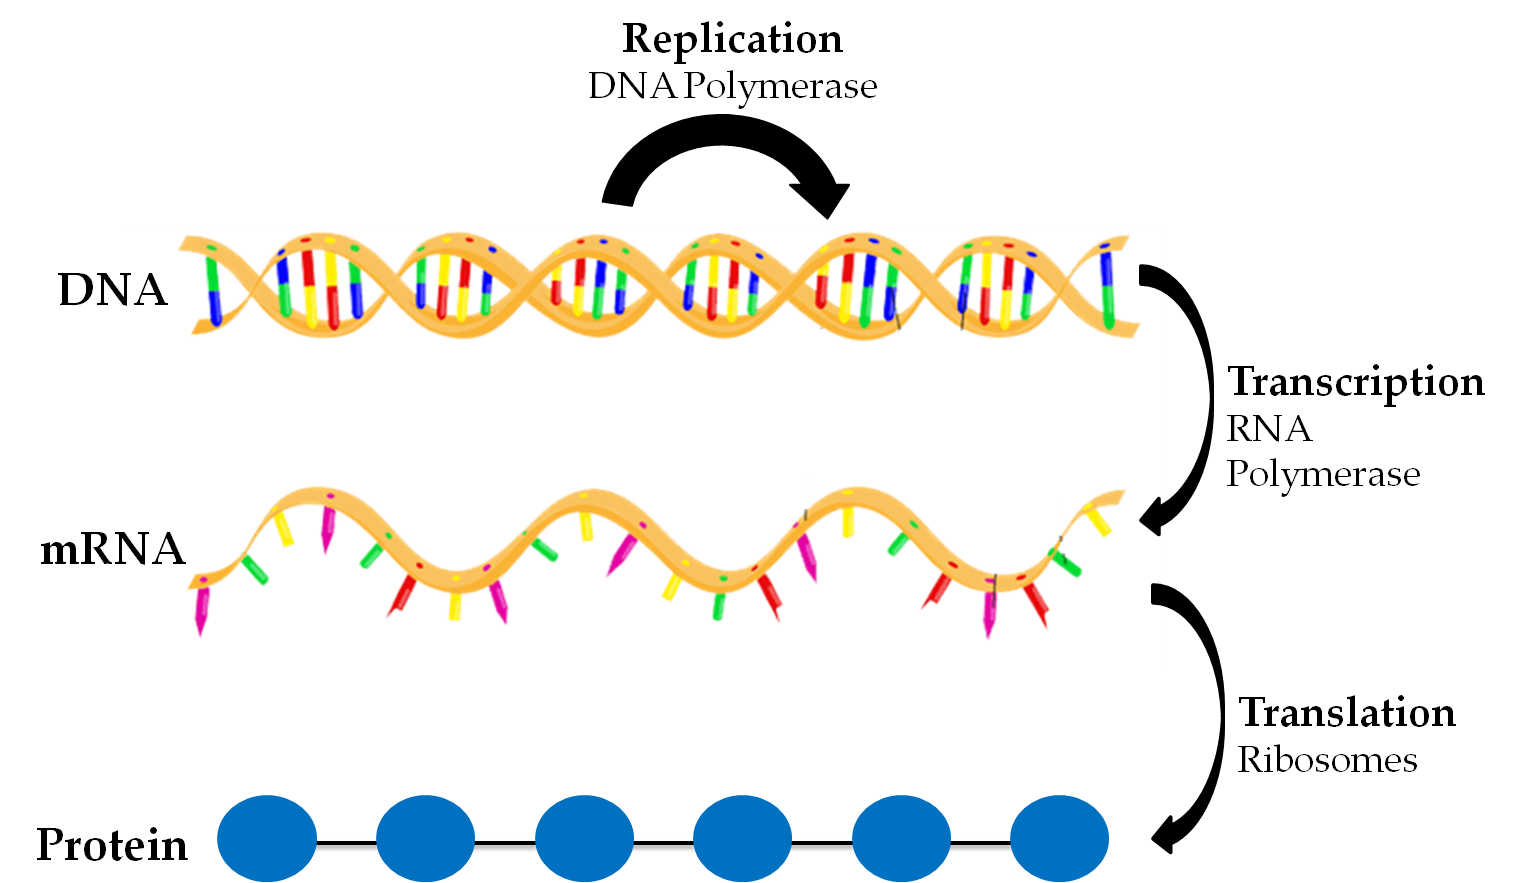
\includegraphics[width=15cm]{con-dogma}
  \caption[Central dogma of molecular biology]{\label{fig:con-dogma} Scheme of the central dogma of molecular biology. By Dhorspool at en.wikipedia, CC BY-SA 3.0, \$3.}
\end{figure}

An important fact is that the central dogma is valid for all the living beings. The encoding of information in DNA and the mechanisms by which proteins are made according to that information, including the genetic code, are very similar between different organisms.

\section{Gene regulation and biological circuits}

DNA contains all the information necessary to build a living being and let him develop his functions. But genetically identical cells may differ a lot. For example, our neurons are very different in form and function than our skin cells, even though they have the same DNA and thus the same genetic information. This differentiation happens because they are expressing different sets of genes. The genetic information encoded in the DNA is called genotype, while the observable characteristics of an organism are called phenotype. In this terminology, both kinds of cells have the same genotype but differ in their genotypes \cite{alberts13} \cite{alon06}.

Those differences lie on the genes that each cell is expressing at a certain time and how much they are being expressed (measured in the rate of production of proteins corresponding to a gene). There are proteins (and even RNA molecules) that inhibit the production of other protein by stoping transcription of the corresponding gene. On the contrary, there are proteins that enhance the production of other proteins by increasing the rate of transcription. Both activators and inhibitors are called \textit{transcription factors}, both cases can be seen on fig. \ref{fig:con-tf_simple}.

\begin{figure}[H]
  \centering
  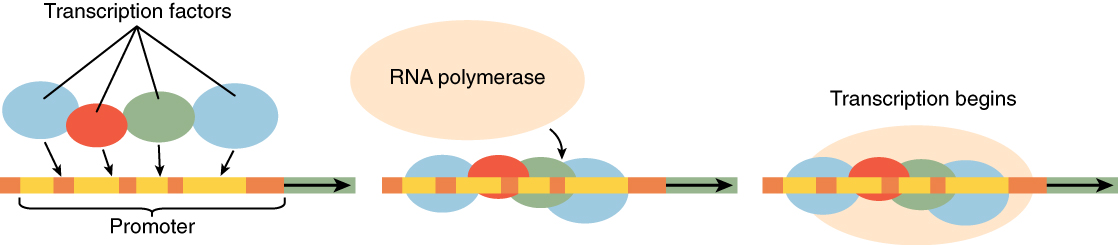
\includegraphics[width=12cm]{con-tf_simple}
  \caption[Transcription factors]{\label{fig:con-tf_simple} Scheme of the mechanisms of transcription factors. Retrieved from: \url{http://biowiki.ucdavis.edu}}
\end{figure}

The mechanisms of gene regulation can be very complex. For example, a molecule can change the conformation of another protein that when affected by the first, inhibits the transcription of certain gene. Those molecules may be signals from the environment and with mechanisms of this type, the cell process environmental signals to express the optimal genes according to the environment. It is also important to point out that the inhibition and activation is not necessarily done individually. A certain gene may need more than one different protein to enhance its activity, or there may be genes that are activated by a protein and inhibited by others, whose production is in turn mediated by other molecules and transcription factors, a well studied case is the \textit{lac} operon in \textit{E. coli} whose mechanism is explained on fig. \ref{fig:con-lac_operon}.

From the biochemical point of view, transcription factors bind specific sites on the \textit{promoter}, a region of the DNA which is upstream the gene (or set of genes for prokaryotes), and it is where the RNA Polymerase binds to initiate transcription (see fig. \ref{fig:con-parts_of_DNA}). The binding of the transcription factor may enhance or obstruct the binding of RNA Polymerase to the promoter. A promoter that is not regulated by transcription factor is called a \textit{constitutive promoter}.

\begin{figure}[H]
  \centering
  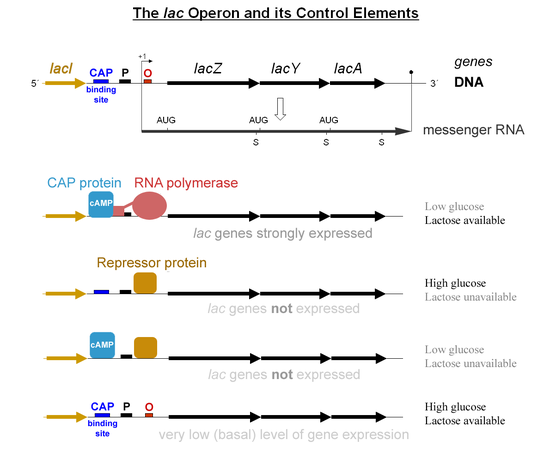
\includegraphics[width=10cm]{con-lac_operon}
  \caption[Example of gene regulation]{\label{fig:con-lac_operon} Example of gene regulation (Lac operon). Retrieved from \url{upload.wikimedia.org/wikipedia/commons/thumb/d/d2/Lac_operon-2010-21-01.png/550px-Lac_operon-2010-21-01.png}}
\end{figure}

\begin{figure}[H]
  \centering
  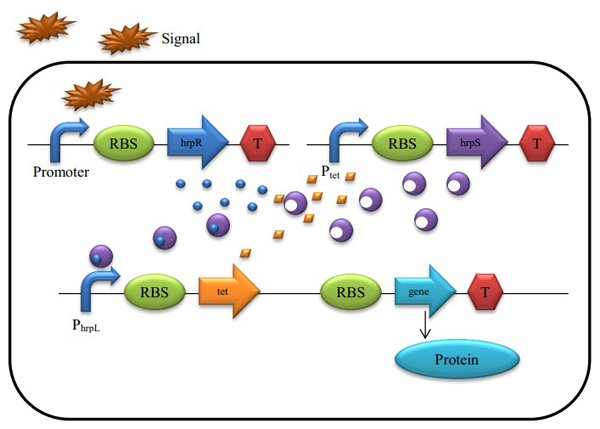
\includegraphics[width=10cm]{con-parts_of_DNA}
  \caption[Parts of a gene]{\label{fig:con-parts_of_DNA} The promoter, RBS, stop codon are shown. Retrieved from \url{http://2013.igem.org/wiki/images/c/c6/HIT-Harbin_Project_Schematic.png}}
\end{figure}

Therefore, in addition to the genotype, gene expression is very important for the cells to develop properly. And, together with the genetic information, defines its structure and behavior. With this in mind, and the fact that those networks may be very large and complex, the approach that Systems Biology is proposing consists on focusing on the interactions between the different genes and components of a cell rather than on the details of the structure of the molecules involved. The set of interactions may be visualized as biological circuits, that are groups of genes that regulate each other's expression. Figure \ref{fig:con-biocircuits_conv} shows some of the conventions used in the schemes of biological circuits.

\begin{figure}[H]
  \centering
  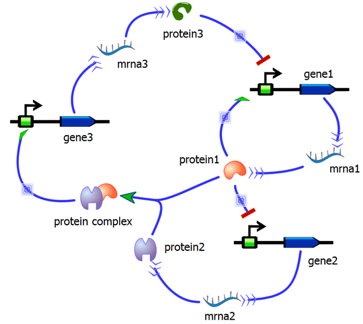
\includegraphics[width=13cm]{con-biocircuits_conv}
  \caption[Systems biology conventions]{\label{fig:con-biocircuits_conv} Typical conventions for biological circuits used in Systems Biology. Retrieved from \url{http://beacon-center.org/wp-content/uploads/2012/10/SyntheticGeneCircuit.png}}
\end{figure}

\begin{figure}[H]
  \centering
  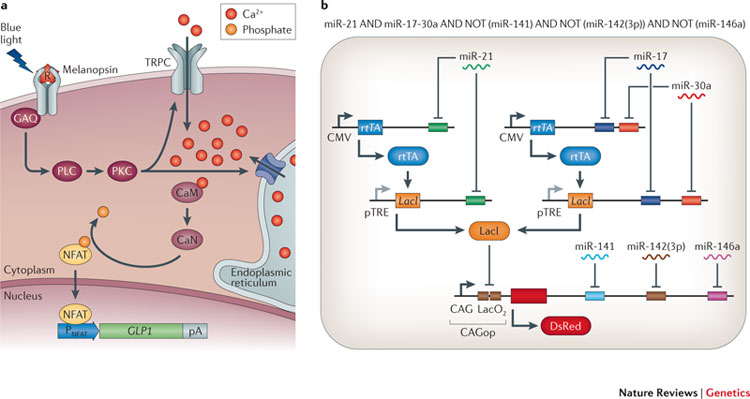
\includegraphics[width=12cm]{con-biocircuits_comp}
  \caption[Example of a biological circuit]{\label{fig:con-biocircuits_comp} Example of a biological circuit. Retrieved from \url{http://www.nature.com/nrg/journal/v13/n6/images/nrg3227-i2.jpg}}
\end{figure}

\section{Hill functions}
\label{sec:hill}

To model the regulation on a gene by a transcription factor, a widely used model is the Hill equation. We will derive it for a particular case that allows a phenomenological understanding of the principles \cite{alon06}.

Consider a transcription factor $X$ that binds to the promoter of some gene, we will label the promoter (gene) as $D$. Also, suppose that $X$ has $n$ binding sites on the promoter and ignore the intermediate states, where less than $n$ molecules of $X$ are bound. The chemical equation is

\begin{equation*}
  \ce{n[X] + [D]} \ce{<=>[k_+][k_-]} \ce{[nXD]}.
\end{equation*}

Hence, $[nXD]$ changes over time as

\begin{equation*}
  \frac{\mathrm{d}[nXD]}{\mathrm{d}t} = k_+[X]^n[D] - k_-[nXD],
\end{equation*}

which in steady state yields

\begin{equation}
  \label{eq:hillss}
  [X]^n[D] = \frac{k_-}{k_+}[nXD].
\end{equation}

Taking the total number $D_T$ of copies of the gene (promoter and DNA molecules) as a constant we obtain

\begin{equation*}
  [D_T] = [D]+[nXD].
\end{equation*}

Solving for the free DNA concentration $[D]$ and replacing in eq. \eqref{eq:hillss}

\begin{equation*}
  [X]^n\left([D_T]-[nXD]\right) = \frac{k_-}{k_+}[nXD].
\end{equation*}

$[nXD]/[D_T]$ and $[D]/[D_T]$ are the fractions of DNA bound and unbound to the transcription factor, respectively, solving for those quantities we obtain

\begin{equation*}
  \frac{[nXD]}{[D_T]} = \frac{[X]^n}{K_d^n+[X]^n}, \quad\quad\quad\quad\quad  \frac{[D]}{[D_T]} = \frac{K_d^n}{K_d^n+[X]^n} = \frac{1}{1+\left(\frac{[X]}{K_d}\right)^n},
\end{equation*}

where $K_d^n \coloneqq k_-/k_+$. In a timescale such that many bindings and unbindings of the transcription factor to the promoter have occurred, those fractions can be interpreted as the probability of having $n$ bound molecules of $X$, and the probability for being unbound, respectively. If the increasing in transcription rate with respect to the basal rate $a$ is proportional to the probabilities of being bound for an activator, and of being unbound for a repressor, the net rates are

\begin{equation}
  \label{eq:con-hillac}
  f([X]) = a + b \frac{[X]^n}{K_d^n+[X]^n},
\end{equation}

for an activator, and

\begin{equation}
  \label{eq:con-hillrep}
  f([X]) = a + b \frac{1}{1+\left(\frac{[X]}{K_d}\right)^n}.
\end{equation}

for a repressor. $b+a$ is the maximum transcription rate, wich happens when $[X]\rightarrow\infty$ for the case of an activator, and when $[X]=0$ for the repressor. $K_d$ is called the \textit{dissociation constant}, which is the concentration of $[X]$ needed for half activation or repression. Biologically it represents the chemical affinity between $x$ and the promoter.  $n$ is called the \textit{Hill coefficient} and from the derivation can be said that it is related to the cooperativity of the transcription factor, being larger if the binding of a molecule of $[X]$ enhances more the binding of another one. A larger value of $n$ give a more step-like Hill function. Figures \ref{fig:con-hill_act} and \ref{fig:con-hill_rep} show the shape of typical Hill functions given by eqs. \eqref{eq:con-hillac} and \eqref{eq:con-hillrep}.

\begin{figure}[H]
  \centering
  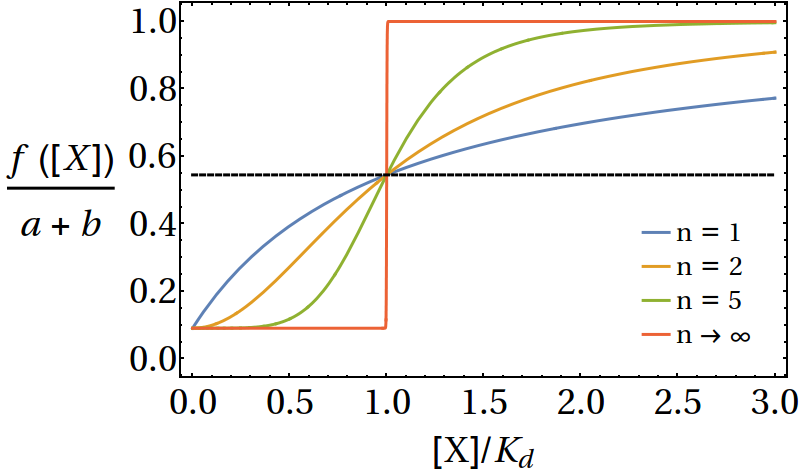
\includegraphics[width=12cm]{con-hill_act}
  \caption[Hill function for an activator]{\label{fig:con-hill_act} Hill functions for an activator. Various values of $n$ are shown. The dashed line shows the point of half activation corresponding to $[X]=K_d$. All have the same value of $K_d$, $a$ and $b$ with $\nicefrac{b}{a}=10$.}
\end{figure}

\begin{figure}[H]
  \centering
  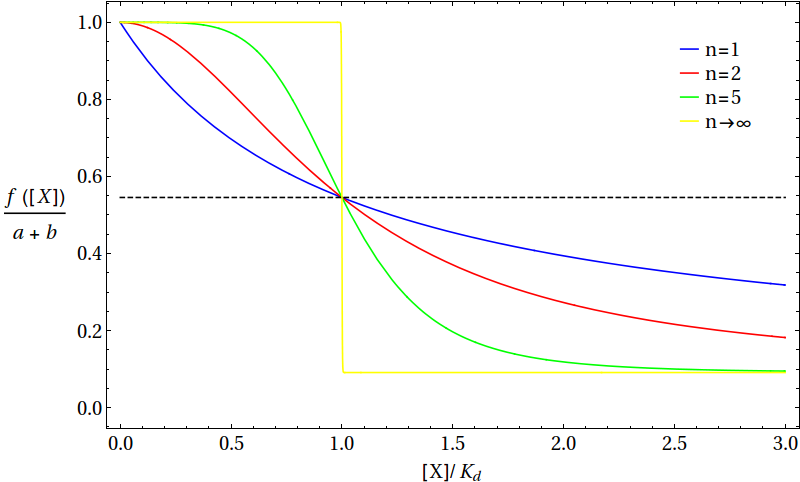
\includegraphics[width=12cm]{con-hill_rep}
  \caption[Hill function for a repressor]{\label{fig:con-hill_rep} Hill functions for a repressor. With the same parameters as fig. \ref{fig:con-hill_act}.}
\end{figure}

Notice in both graphs that as $n\rightarrow\infty$, the function appears more like a Heaviside function with the step in $[X] = K_d$. This approximation can be very useful on a first qualitative analysis of biological circuits but such high values of $n$ are biologically unrealistic. The case $n=1$ corresponds to the Michaelis-Menten equation.

\section{Probability}

Consider an experiment in which the set of possible outcomes is clearly known. A random variable $X$ is a quantity that can take values from that set of possible outcomes $\{x\}$ of the experiment. How likely is that any value $x$ happens in a given trial of the experiment is determined by the probability mass function (PMF) $P(x)$ if the variable is discrete. For a discrete random variable, $P(x)$ represents the fraction of trials of the experiment in which $X$ has the value $x$ when the number of trials is large. The PMFs follow the axioms of nonnegativity, additivity and normalization. \cite{bertsekas08} \footnote{We will focus here on discrete random variables. The continous case is very similar, it reduces almost entirely to change $\sum$ by $\int\mathrm{d}x$ and $P(x)$ by $\rho(x)$, where $\rho(x)$ is the probability density function (PDF), the analogous of the PMF.} 

For several random variables $X_1,\dotsc,X_n$, the joint PMF  $P(x_1,\dotsc,x_n)$ is defined as the probability that $X_1=x_1,\dotsc,X_n=x_n$. The set of random variables are \textbf{independent} if

\begin{equation*}
  P(x_1,\dotsc,x_n) = P(x_1)\dotsm P(x_n)
\end{equation*}

The conditional probability of the r. v.s $X_1,\dotsc,X_k$ given the variables $X_{k+1},\dotsc,X_n$ is denoted by $P(x_1,\dotsc,x_k|x_{k+1},\dotsc,x_n)$ and it is defined as

\begin{equation*}
  P(x_1,\dotsc,x_k|x_{k+1},\dotsc,x_n) \coloneqq \frac{P(x_1,\dotsc,x_n)}{P(x_{k+1},\dotsc,x_n)},
\end{equation*}

provided that the denominator is different from $0$. It can be thought as the probability of a certain outcome for $x_1,\dotsc,x_k$ when certain given values of $x_{k+1},\dotsc,x_n$ have been obtained. Notice that if all the random variables are independent it reduces to

\begin{equation*}
  P(x_1,\dotsc,x_k|x_{k+1},\dotsc,x_n) = P(x_1,\dotsc,x_k).
\end{equation*}

The conditional and unconditional probabilities are equal, meaning that the outcome of $(x_{k+1},\dotsc,x_n)$ does not affect the outcome of $(x_1,\dotsc,x_k)$.

To find the probability of a certain outcome of $X$, sometimes it is easier to use the \textbf{total probability theorem}

\begin{equation*}
  P(x) = \sum_y P(x,y) = \sum_y P(x|y)P(y).
\end{equation*}

The \textbf{expected value} (also called average) of a function of a random variable $f(X)$ is defined as

\begin{equation}
  \label{eq:con-ave_def}
  \langle f(X)\rangle \coloneqq \sum_xf(x)P(x).
\end{equation}

From the definition can be noticed that the expected value is linear, i.e., for a pair of random variables $X$ and $Y$, and a constant $c$

\begin{equation*}
  \langle X+cY\rangle = \langle X\rangle+c\langle Y\rangle.
\end{equation*}

The variance $\sigma^2(X)$ of $X$ measures the dispersion of the possible outcomes of the random variable, it is defined as

\begin{equation*}
  \sigma^2(X) \coloneqq \left\langle\left( X-\langle X\rangle\right)^2\right\rangle.
\end{equation*}

It can be easily shown that

\begin{equation}
  \label{eq:con-var_nice}
  \sigma^2(X) = \langle X^2\rangle - \langle X\rangle^2.
\end{equation}

From the previous equation it can be seen that for a constant $c$

\begin{equation}
  \label{eq:con-var_const}
  \sigma^2(cX) = c^2\sigma^2(X)
\end{equation}

The $\mathbf{n}$\textbf{th moment} of the random variable $X$ is given by

\begin{equation*}
  \langle X^n\rangle \coloneqq \sum_xx^nP(x).
\end{equation*}

Hence, the expected value is the first moment and the variance can be written in terms of the first and second moments.

If $X$ and $Y$ are independent, it can be shown that

\begin{equation}
  \label {eq:con-mom_ind}
  \langle XY\rangle = \langle X\rangle\langle Y\rangle \quad\text{and}\quad \sigma^2(X+Y) = \sigma^2(X)+\sigma^2(Y).
\end{equation}

The conditional expectation of $X$ given a random variable $Y$, $\langle X|Y\rangle$ is itself a random variable which depends on $Y$, which when $Y$ is fixed in some $y$ is given by

\begin{equation*}
  \langle X|y\rangle \coloneqq \sum_xxP(x|y),
\end{equation*}

and it follows that

\begin{equation}
  \label{eq:con-total_exp}
  \left\langle\langle X|Y\rangle\right\rangle = \left\langle X\right\rangle
\end{equation}

which is the \textbf{law of total expectation}, for the variance there is an analogous theorem, called the \textbf{law of total variance}

\begin{equation}
  \label{eq:con-total_var}
  \sigma^2(x) = \left\langle\sigma^2(x|y)\right\rangle + \sigma^2\left(\langle x|y\rangle\right)
\end{equation}

The \textbf{covariance} of $X$ and $Y$ is defined as

\begin{equation*}
  \text{cov}(X,Y) \coloneqq \left\langle\left(X-\langle X\rangle\right)\left(Y-\langle Y\rangle\right)\right\rangle = \langle XY\rangle - \langle X\rangle\langle Y\rangle.
\end{equation*}

It can be thought as a measure of how correlated is their behaviour. For example, if the value of $Y$ is known, the value of $X$ will be more likely to be known if the covariance is high in absolute value. The covariance will be $0$ if it does not give us any information. Consider the extreme case, if $Y=X$, $\text{cov}(X,X) = \sigma^2(X)$, while if $X$ and $Y$ are independent by eq. \eqref{eq:con-mom_ind} we get $\text{cov}(X,Y) = 0$.

\section{Noise}
\label{sec:con-noise}
Intuitively, we may expect that a random variable is more 'random' or noisy, when the deviations relative to the expected value are bigger. With this in mind, the noise in a random variable $X$ must increase as the variance increases and decrease as the mean increases (the same deviation from a smaller expected value contributes more to the noise than from a bigger one). The quantities that have benn used to measure noise in biology are the Fano factor $\nu$ and the coefficient of variation $\eta$, which are defined by

\begin{equation}
  \label{eq:con-fano_def}
  \nu_X \coloneqq \frac{\sigma^2(X)}{\langle X \rangle}.
\end{equation}

\begin{equation}
  \label{eq:con-cv_def}
  \eta_X \coloneqq \frac{\sigma(X)}{\langle X \rangle}.
\end{equation}

The Fano factor has been used in the first studies of noise in biology since it had the particular property that for a random variable with a Poisson distribution $\nu_X=1$ and hence it measures deviations from a Poissonian behavior. In more recent studies the coefficient of variation is being used because it is dimensionless and for that reason it does not depend on the units used for the random variable. For this reason, the generic term 'noise' is now used to refer to $\eta$.

\section{Moment generating functions}

Let $n_1,\dotsc,n_N$ be discrete random variables over $\mathbb{N}$ and let $f(n_1,\dotsc,n_N)$ be the joint probability mass function. The moment generating function $F(z_1,\dotsc,z_N)$ is defined as \footnote{Not to be confused with the cumulative distribution function}

\begin{equation}
  \label{def:mom_gen}
  F(z_1,\dotsc,z_N) \coloneqq \sum_{\mathclap{n_1=0}}^{\infty} \dotsi \sum_{\mathclap{n_N=0}}^{\infty} z_1^{n_1} \dotsm z_N^{n_N} f(n_1,\dotsc,n_N).
\end{equation}

Evaluating the function on $z_1 = \dotsb = z_N = 1$ (denoted by $\left. \right|_1$) we obtain

\begin{equation}
  \label{eq:con-mom_gen_1}
  \left.F\right|_1 = \sum_{\mathclap{n_1,\dotsc,n_N}}f(n_1,\dotsc,n_N) = 1.
\end{equation}

by the axiom of normalization. Taking the derivative of eq. \ref{def:mom_gen} with respect to $z_i$, $i = 1,\dotsc,N$ we get

\begin{equation}
  \label{eq:con-mom_gen_d1}
  \left.\frac{\partial F}{\partial z_i}\right|_1 = \left.\sum_{\mathclap{n_1,\dotsc,n_N}}n_i z_1^{n_1}\dotsm z_i^{n_i-1}\dotsm z_N^{n^N}f(n_1,\dotsc,n_N)\right|_1 = \sum_{\mathclap{n_1,\dotsc,n_N}} n_i f(n_1,\dotsc,n_N) = \langle n_i \rangle.
\end{equation}

Differentiating again with respect to $z_j$, $j=1,\dotsc,N$ with $j\neq i$ we obtain

\begin{equation}
  \label{eq:con-mom_gen_d1d2}
  \left. \frac{\partial F}{\partial z_i z_j} \right|_1 = \langle n_i n_j \rangle.
\end{equation}

Differentiating eq. \ref{def:mom_gen} twice with respect to $z_i$ we obtain similarly

\begin{equation}
  \label{eq:con-mom_gen_d1d1}
  \left. \frac{\partial^2F}{\partial z_i^2}\right|_1 = \langle n_i(n_i-1) \rangle.
\end{equation}

These properties will be very useful in the next sections to find the noise of a genetic system.

\section{Characteristic function}
\label{sec:con-charac_func}
Another transformation of the PMF that has properties similar to the mentioned for the moment generating function is the characteristic function. It is defined for a $N$-tuple of random variables $(X_1,\dotsc,X_N)$ as\footnote{We will consider here the case with the real exponent}.

\begin{equation*}
  \phi(s_1,\dotsc,s_N)\coloneqq \left\langle e^{\sum_{i=1}^Ns_ix_i}\right\rangle = \sum_{x_1}\dotsi\sum_{x_N}\exp\left(\sum_{i=1}^Ns_ix_i\right).
\end{equation*}

We will denote the evaluation at $s_1=\dotsb=s_N=0$ by $|_0$ It is easy to see that by normalization

\begin{equation*}
  \phi(s)|_0 = 1.
\end{equation*}

Differentiating once with respect to $s_i$ for $i=1,\dotsc,N$.

\begin{equation}
  \label{eq:con-char_1}
  \left.\frac{\partial\phi(s_1,\dotsc,s_N)}{\partial s_i}\right|_0 = \left.\left\langle x_i e^{\sum_{i=1}^Ns_ix_i}\right\rangle\right|_0 = \langle x_i\rangle.
\end{equation}

Each differentiation with respect to $s_i$ produces a factor $x_i$ in the average, hence

\begin{equation}
  \label{eq:con-char_2}
  \left.\frac{\partial^2\phi(s_1,\dotsc,s_N)}{\partial s_i \partial s_j}\right|_0 = \langle x_ix_j\rangle.
\end{equation}

This equation is valid for any $i,j=1,\dotsc,N$, even for the case $i=j$. In that case the right hand side becomes $\langle x_i^2\rangle$. By calculating higher order derivatives we can find higher order moments in the same way.
  
\section{Stochastic processes}

A stochastic process $X(t)$ \footnote{or $\{X\}_n$ if the time steps are discrete} is a set of random variables indexed by another variable, which usually is taken to be the time. An outcome of the stochastic process is a function of time which varies randomly between different repetitions of the experiment \cite{vankampen92} \cite{gardiner03}.

The \textbf{autocorrelation} $C_X$ of a stochastic process $X(t)$ is given by

\begin{equation*}
  C_X(t,t') \coloneqq \langle X(t)X(t')\rangle.
\end{equation*}

It measures the degree of correlation between outcomes of the random variables at different times. If the process $X$ is \textbf{stationary}, the autocorrelation only depends on the time difference, i.e.

\begin{equation*}
  C(\tau) \coloneqq \langle X(t)X(t+\tau)\rangle,
\end{equation*}

where $\tau \coloneqq t'-t$.

The \textbf{power spectrum} $S_X$ of a stochastic process is defined as average of the square norm of its the Fourier transform

\begin{equation*}
  S_X(\omega) \coloneqq \left|\langle\hat X\rangle\right|^2,
\end{equation*}

where the hat denotes Fourier transform. A mathematical tool that will be very useful in the calculations is the \textbf{Wiener-Khinchin theorem} It states that the power spectrum and the autocorrelation are Fourier-Transform pairs, that is

\begin{equation}
  \label{eq:con-wkth}
  \mathscr{F}(C_X(\tau)) = S_X(\omega),\quad\text{and}\quad \mathscr{F}^{-1}(S_X(\omega)) = C_X(\tau).
\end{equation}

\section{The Poisson process}
\label{sec:poisson}

Many of the processes of creation and destruction that occur in this context are modeled as Poisson processes. For example, the creation and destruction of mRNA and proteins.The Poisson process is a continous-time stochastic process that is used to model arrivals when there is some known arrival rate and when the arrivals at different time intervals are independent.

Mathematically, we define $P(k,\tau)$ as the probability that there are $k\in\mathbb{Z}$ arrivals during a time interval $\tau$ and assume that it is the same for any interval of the same length. We denote by $\lambda$ the arrival rate for the process. The Poisson process satisfy the following properties

\begin{itemize}
  \item  $P(k,\tau)$ is the same for all intervals of length $\tau$.
  \item  The value of $P(k,\tau)$ during some particular interval is independent of other intervals.
  \item $P(k,\tau)$ satisfies the following
    \begin{equation*}
      \begin{split}
        P(0,\tau)=1-\lambda\tau+o_0(\tau),\\
        P(1,\tau)=\lambda\tau+o_1(\tau),\\
        P(k,\tau)=o_k(\tau).\quad\text{for } k>1.
      \end{split}
    \end{equation*}
    
    Where $o_k(\tau)$, $k=0,1,\dotsc$ are functions that become negligible compared to $\tau$ as it becomes small, that is

    \begin{equation*}
      \lim_{\tau\to 0}\frac{o_k(\tau)}{\tau}=0.
    \end{equation*}
\end{itemize}

According to the previous properties, $P(k,\tau)$ is given by

\begin{equation*}
  P(k,\tau) = e^{-\lambda\tau}\frac{(\lambda\tau)^k}{k!},\quad k=0,1,\dotsc
\end{equation*}

which is a Poisson PMF, using the definition for the expected value and variance (eqs. \eqref{eq:con-var_nice} and \eqref{eq:con-ave_def}), letting $N_\tau$ be the number of arrivals during a time interval $\tau$  we get after a little algebra

\begin{equation*}
  \langle N_\tau\rangle = \sigma^2(N_\tau) = \lambda \tau.
\end{equation*}

The average number of arrivals in a time $\tau$ is, as intuitively expected, the arrival rate times the length of the interval. From eqs. \eqref{eq:con-fano_def} and \eqref{eq:con-cv_def}, the noise and Fano factor for $N_\tau$ are

\begin{equation}
  \label{eq:con-poisson_noise}
  \nu(N_\tau) = 1,\quad\quad \eta(N_\tau) = \frac{1}{\sqrt{N_\tau}}.
\end{equation}

This proves what was said on section \ref{sec:con-noise} about the previous use of the Fano factor as the standard measure of noise. From the form of $\eta$ we conclude that if the number of events is large, the Poisson noise is negligible. But for a biological system, for instance, the average number of copies of mRNA of a given gene is of the order of $10$. This makes the effect of noise a significant factor. Also, altought the mean number of proteins is of the order of $1000$, the Poisson noise is negligible, but there is an important contribution of noise coming from the RNA and other sources, as we will see on chapter \ref{ch:master}.

Now we will find the time between events, by now let $t=0$ the time of the last event and let $t=T$ the time of the next event, then

\begin{equation*}
  P(T\leq t) =\int_0^tf_T(t')dt'=1-P(T>t) = 1 - P(0,t) = 1 - e^{-\lambda t}.
\end{equation*}

Differentiating and applying the fundamental theorem of calculus, we get the \textbf{exponential PDF}, which is given by

\begin{equation*}
  \label{eq:con-exp_pdf}
  f_T(t) = \lambda e^{-\lambda t}.
\end{equation*}

Therefore, the time $T$ until the first arrival follows an exponential distribution. 

The exponential distribution is \textbf{memoryless} in the following sense: suppose an arrival happened at time $t'$, therefore, the probability distribution for the remaining time until the next arrival is an exponential with the same rate. With this in mind, not only the time until the first arrival, but all the interarrival times (the times between arrivals), follow the distribution given by eq. \eqref{eq:con-exp_pdf}.

Suppose we $k$ independent Poisson processes with rates $\lambda_1,\dotsc,\lambda_k$ and we record an arrival each time an arrival occur in either process. This merged process is also a Poisson process with rate $\Lambda\coloneqq\sum_{i=1}^k\lambda_i$. Also, any arrival of the merged process has a probability $\lambda_i/\Lambda$, $i=1,\dotsc,k$ of being an arrival of the $i$th process.

In the models we will consider there might be several creation and destruction events which are Poissonian and independent, for example, the synthesis and degradation of different kinds of RNA and protein, the binding of transcription factors, etc. For these models, we can take advantage of the merging properties of Poisson processes to make efficient and precise simulations.

\section{The Gillespie algorithm}

To simulate the models we will use the Gillespie algorithm \cite{gillespie77} which improves speed a lot with respect to brute-force stochastic algorithms. It is used to simulate simultaneous Poissonian events that occur with a certain rate (probability per unit time), e.g. synthesis and degradation of RNA or proteins, binding of an enzyme to a substrate, etc.

In the brute-force approach we consider a fixed time interval that must be sufficiently small, and for every possible event we sample a random number that depending on the probabilities of the events, will tell us which of the events happened or if nothing happened at that interval. This procedure is repeated for all the intervals. Since time intervals must be small and for each interval we must sample as many random numbers as events, this approach is computationally inefficient.

In the Gillespie algorithm, we take advantage of the mentioned properties of the Poisson process \cite{bertsekas08}. There are not fixed time intervals in this case, a random number is sampled with an exponential distribution whose rate $\Lambda$ is the sum of the rates of the individual processes to find the time of occurence of the next event and another uniform one is sampled to evaluate which of the events occured. Using the properties of the exponential CDF, to sample an exponential random number $X$ with parameter $\Lambda$ from an uniform $U$ between $0$ and $1$ we apply the following equation

\begin{equation}
  X = -\frac{1}{\Lambda}\ln(U).
\end{equation}

The Gillespie algorithm is by far more efficient. First, it does not need to have a fixed small time interval, it finds the time intervals between events. Second, the number of random numbers sampled per time interval in the brute-force approach is equal to the number of events (which can be large), and many of the intervals there will not be an event, while in the Gillespie algorithm only two random numbers are sampled by event and the way in which the time interval is sampled allows to go forward in time in many fewer steps. Finally, a very important aspect is that the Gillespie algorithm is that it is exact, while the precision of the brute-force algorithm depends on how small is the time interval in consideration.

\chapter{Basic genetic circuits in steady state - The master equation}
\label{ch:master}

In this chapter, we develop a model of a genetic system considering only its intrinsic noise using the master equation, which is an approach to model stochastic processes where there are defined states and there are certain transition probabilities between states.

This chapter is based on the work done by M. Thattai and A. van Oudenaarden in \cite{thattai01}.

\section{Single gene}

For the process of transcription and translation the number $d$ of DNA copies of certain gene is taken to be constant and the rate $k_r$ of production of RNA ($n_1$) is proportional to $d$. In the same way, the rate $k_p$ of production of proteins ($n_2$) per mRNA is constant. There is also a degradation rate for each molecule proportional to their concentration. The model is ilustrated in fig. \ref{fig:mas-dogma}.

\begin{figure}[H]
  \centering
  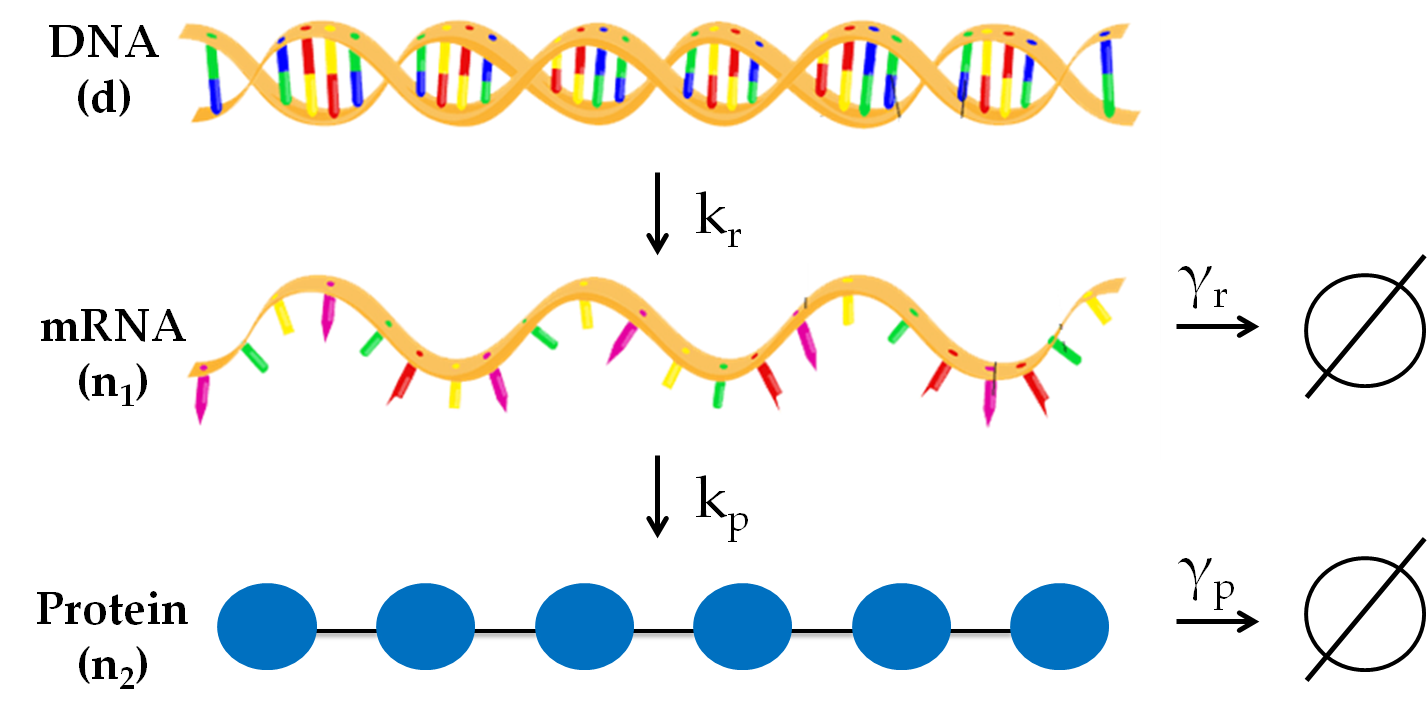
\includegraphics[width=8cm]{mas-dogma}
  \caption[Model of gene expression for a single gene]{\label{fig:mas-dogma} Steps of gene expression considered in the model. Taken from \cite{thattai01}.}
\end{figure}

The deterministic equations describing these processes are therefore given by

\begin{align}
  \dot{n_1}(t) &= k_rd-\gamma_rn_1(t)\label{eq:mas-simple_det_1},\\
  \dot{n_2}(t) &= k_pn_1(t)-\gamma_pn_2(t) \label{eq:mas-simple_det_2}.
\end{align}

Hence, on steady state

\begin{align}
  \langle n_1 \rangle &= \frac{k_r}{\gamma_r} \label{eq:mas-simple_ss_1}, \\
  \langle n_2 \rangle &= \frac{k_p}{\gamma_p} \langle n_1 \rangle = \frac{k_pk_r}{\gamma_p\gamma_r} \label{eq:mas-simple_ss_2}.
\end{align}

But these are numbers of molecules which are discrete, and on that discreteness lies part of the stochastic behaviour of those kind of systems. The molecules are created and degradated one at a time at a certain average rate but the timing between each creation or degradation should not match exactly the rates. 

To model the intrinsic noise, we will consider each pair of values of $(n_1,n_2)$ as a possible state for the system. There are transitions between the possible states which are proportional to the rates of creation and degradation as can be seen on figure \ref{fig:mas-trans_single}.

\begin{figure}[H]
  \centering
  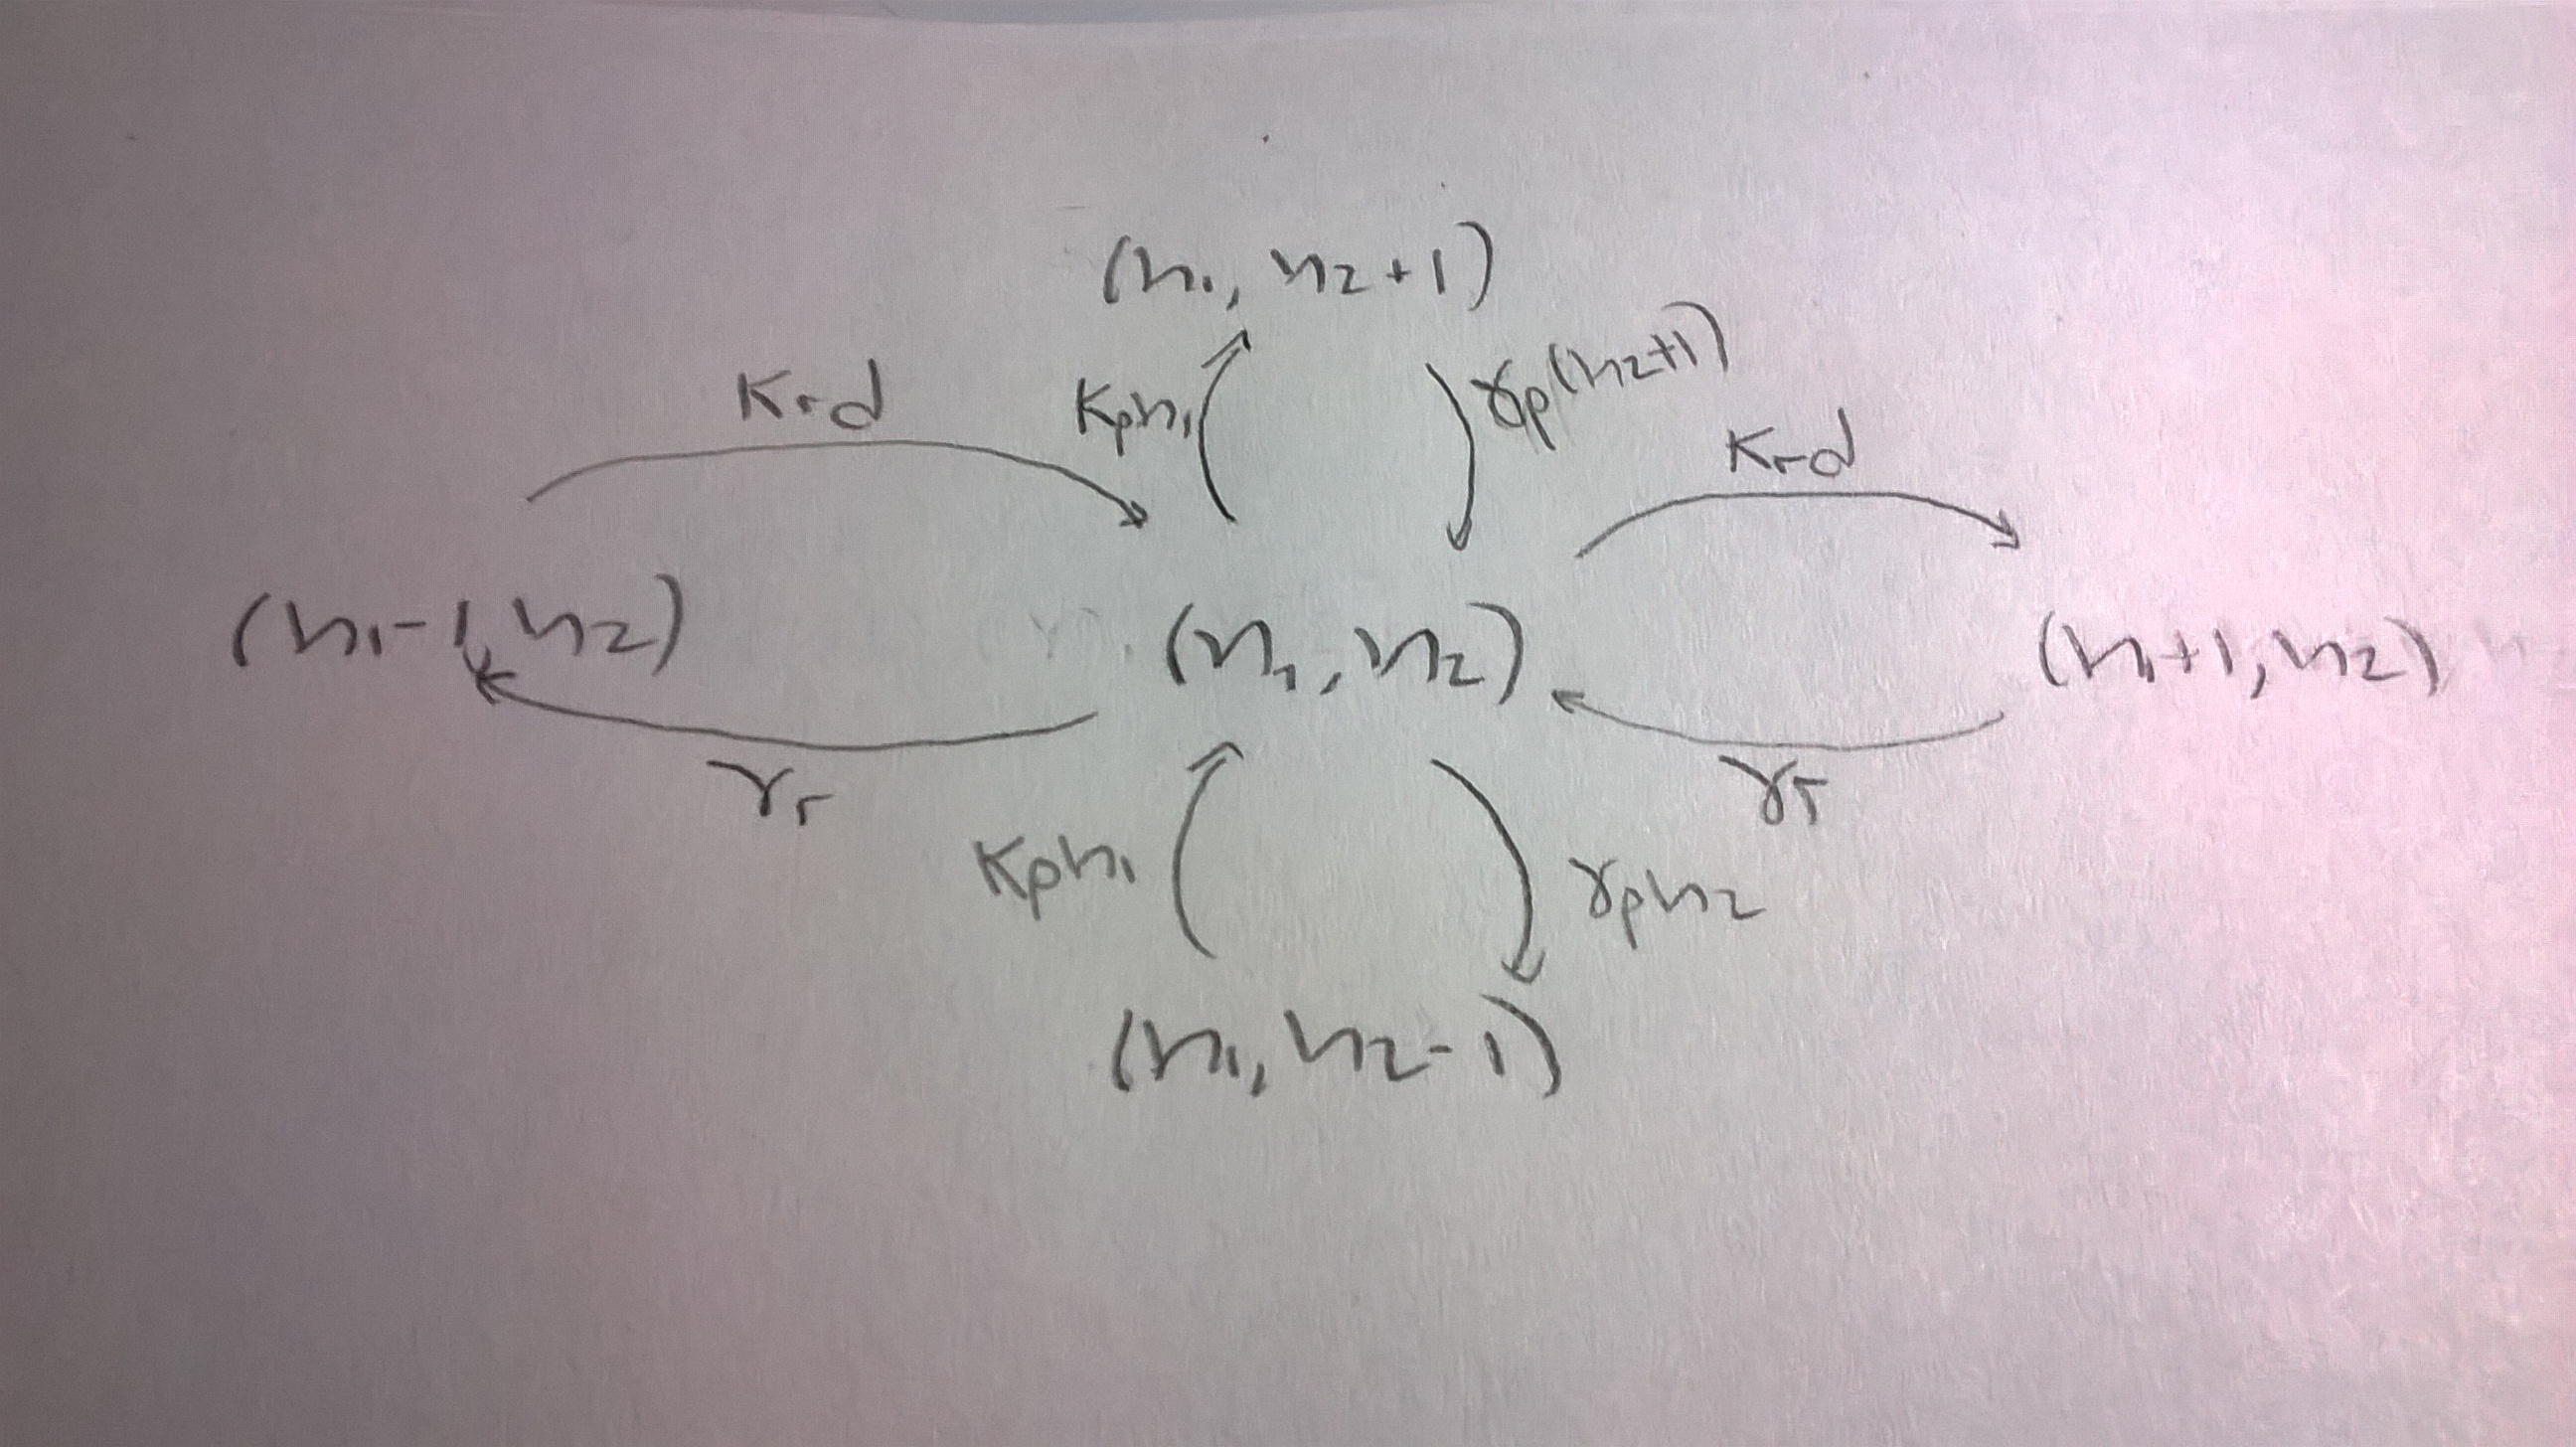
\includegraphics[width=8cm]{mas-trans_single}
  \caption[Transitions between states for a single gene]{\label{fig:mas-trans_single} Scheme of the possible transitions involving $n_1$ RNA molecules and $n_2$ protein molecules.}
\end{figure}

The transitions shown in figure \ref{fig:mas-trans_single} are the ways in which $(n_1,n_2)$ can change. This transitions can be interpreted probabilistically. There is a probability $p(n_1,n_2,t)$ of being at the state $(n_1,n_2)$ at time $t$ which changes according to the probabilities of being in the adjacent states and the transition probabilities given by the reaction rates. The reaction rates are interpreted as the probabilities per unit time for a reaction to occur. For instance, in a small time $\mathrm{d}t$, the probability of creating a mRNA molecule is $k_r\mathrm{d}t$. For the other it is analogous. Also, it is assumed that the probabilities $p$ of being at a state are independent of the transition probabilities.

With this in mind, we can write a difference-differential equation for the probability distribution $p$ which is called the master equation. It is a difference equation in the number of species $(n_1,n_2)$, and differential in time $t$. In this case it is given by

\begin{equation}
  \label{eq:master}
  \begin{split}
    \frac{\mathrm{d}p(n_1,n_2,t)}{\mathrm{d}t} &= k_rdp(n_1-1,n_2,t) - k_rdp(n_1,n_2,t)\\
&+ k_pn_1p(n_1,n_2-1,t) - k_pn_1p(n_1,n_2,t)\\
&+ \gamma_r(n_1+1)p(n_1+1,n_2,t) - \gamma_rn_1p(n_1,n_2,t)\\
&+ \gamma_p(n_2+1)p(n_1,n_2+1,t) - \gamma_pn_2p(n_1,n_2+1,t)
  \end{split}
\end{equation}

Notice that the first term refers to a transition from state $(n_1-1,n_2,t)$ to $(n_1,n_2,t)$ by a creation of a mRNA molecule, whereas the second term involves a transition $(n_1,n_2,t) \rightarrow (n_1+1,n_2,t)$ also by mRNA synthesis. The third and fourth terms have the meaning but related to protein synthesis. The other terms are related to transitions due to degradation.

We will write the master equation in terms of the moment generating function $F(z_1,z_2)$, as defined in eq. \eqref{def:mom_gen} on page \pageref{def:mom_gen}. Multiplying by $z_1^{n_1}z_2^{n_2}$ and summing over $n_1$ and $n_2$, both from $0$ to $\infty$ we obtain for the left hand side simply $\dot{F}(z_1,z_2)$. For the first term on the right hand side we obtain \footnote{The time dependence is not shown for simplicity.}

\begin{equation*}
  \sum_{\mathclap{n_1=0,n_2=0}}^\infty z_1^{n_1}z_2^{n_2}f(n_1-1,n_2) = \sum_{\mathclap{n_1=-1,n_2=0}}z_1^{n_1+1}z_2^{n_2}f(n_1,n_2),
\end{equation*}

but since $n_1$ represents number of molecules, it must be a positive quantity. Hence $f(-1,n_2)=0$ and the last sum can be taken from $n_1=0$ yielding

\begin{equation*}
  z_1 \sum_{\mathclap{n_1=0,n_2=0}}z_1^{n_1}z_2^{n_2}f(n_1,n_2) = z_1F(z_1,z_2).
\end{equation*}

For the second term of eq. \eqref{eq:master} the result is trivial, for the third term we get

\begin{equation*}
  \sum_{\mathclap{n_1=0,n_2=0}}n_1f(n_1,n_2-1) = \sum_{\mathclap{n_1=0,n_2=-1}}n_1z_1^{n_1}z_2^{n_2+1}f(n_1,n_2).
\end{equation*}

Using the same argument as above, $f(n_1,-1) = 0$. Rearranging it becomes

\begin{equation*}
  z_1 z_2 \sum_{\mathclap{n_1=0,n_2=0}} z_1^{n_1-1}z_2^{n_2}f(n_1,n_2) = z_1 z_2 \frac{\partial F(z_1,z_2)}{\partial z_1}.
\end{equation*}

For the fifth term

\begin{equation*}
  \begin{split}
    \sum_{\mathclap{n_1=0,n_2=0}}(n_1+1)z_1^{n_1}z_2^{n_2}f(n_1+1,n_2) &= \sum_{\mathclap{n_1=1,n_2=0}}n_1z_1^{n_1-1}z_2^{n_2}f(n_1,n_2)\\ 
    &= z_1 \sum_{\mathclap{n_1=0,n_2=0}}n_1z_1^{n_1-1}z_2^{n_2}f(n_1,n_2) = \frac{\partial F(z_1,z_2)}{\partial z_1}.
  \end{split}
\end{equation*}

The other terms are treated in a similar fashion. Putting all of this together in we obtain the master equation in terms of the moment generating function $F$

\begin{equation}
  \label{eq:masterF}
  \begin{split}
    \dot{F}(z_1,z_2,t) &= k_rd(z_1-1)F(z_1,z_2,t) + k_pz_1(z_2-1)\frac{\partial F(z_1,z_2,t)}{\partial z_1} \\
    &+ \gamma_r(1-z_1)\frac{\partial F(z_1,z_2,t)}{\partial z_1} + \gamma_p(1-z_2)\frac{\partial F(z_1,z_2,t)}{\partial z_2}.
  \end{split}
\end{equation}

We thus transformed a difference equation in $(n_1,n_2)$ into a partial differential equation in $(z_1,z_2)$. Instead of solving completely, we will use the properties of $F$ (eqs. \eqref{eq:con-mom_gen_1} - \eqref{eq:con-mom_gen_d1d1}) to find the moments. Taking the derivative with respect to $z_1$ we obtain

\begin{equation}
  \label{eq:dz1}
  \begin{split}
    \frac{\partial \dot{F}}{\partial z_1} &= k_rd\left( F+(z-1)\frac{\partial F}{\partial z_1} \right) + k_p(z_2-1) \left( \frac{\partial F}{\partial z_1} + z_1 \frac{\partial^2 F}{\partial z_1^2} \right)\\
    &+\gamma_r\left(-\frac{\partial F}{\partial z_1}+(1-z_1)\frac{\partial^2 F}{\partial z_1^2}\right)+\gamma_p(1-z_2)\frac{\partial^2 F}{\partial z_1 \partial z_2},
  \end{split}
\end{equation}

and taking the derivative of eq. \eqref{eq:masterF} with respect to $z_2$

\begin{equation}
  \label{eq:dz2}
  \begin{split}
    \frac{\partial \dot{F}}{\partial z_2}&=k_rd(z_1-1)\frac{\partial F}{\partial z_2} + k_pz_1\left(\frac{\partial F}{\partial z_1} + (z_2-1)\frac{\partial^2 F}{\partial z_1 \partial z_2} \right)\\
    &+ \gamma_r(1-z_1)\frac{\partial^2 F}{\partial z_1 \partial z_2} + \gamma_p\left(-\frac{\partial F}{\partial z_2}+(1-z_2)\frac{\partial^2 F}{\partial z_2^2}\right).
  \end{split}
\end{equation}

Evaluating eqs. \eqref{eq:dz1} and \eqref{eq:dz2} at $z_1 = z_2 = 1$ and using properties \eqref{eq:con-mom_gen_1} and \eqref{eq:con-mom_gen_d1} we obtain

\begin{align*}
\dot{\langle n_1 \rangle}&= k_rd - \gamma_r \langle n_1 \rangle,\\
\dot{\langle n_2 \rangle}&= k_p\langle n_1 \rangle - \gamma_p \langle n_2 \rangle.
\end{align*}

Therefore, the averages follow the deterministic equations given by eqs. \eqref{eq:mas-simple_det_1} and \eqref{eq:mas-simple_det_2}. The steady state values are thus given by eqs. \eqref{eq:mas-simple_ss_1} and \eqref{q:mas-simple_ss_2}. The deterministic equations reproduce the average behavior.

Differentiating eq. \eqref{eq:dz1} with respect to $z_2$, eq. \eqref{eq:dz1} with respect to $z_1$ and eq. \eqref{eq:dz2} with respect to $z_2$ and evaluating at $z_1 = z_2 = 1$ we obtain, respectively

\begin{align}
  \dot{\langle n_1n_2\rangle} &= k_rd\langle n_2 \rangle + k_p\left(\langle n_1\rangle + \langle n_1(n_1-1) \rangle \right) - \left( \gamma_r + \gamma_p \right)\langle n_1n_2 \rangle,\label{eq:dz1z2}\\
  \dot{\langle n_1(n_1-1)\rangle} &= 2k_r\langle n_1\rangle-2\gamma_r\langle n_1(n_1-1) \rangle, \label{eq:dz1z1}\\
  \dot{\langle n_2(n_2-1)\rangle} &= 2k_p\langle n_1n_2 \rangle - 2\gamma_p\langle n_2(n_2-1)\rangle. \label{eq:dz2z2}
\end{align}

We will treat the previous equations in steady state, that is, with their time derivatives equal to zero. From  eq. \eqref{eq:dz1z1}, we get

\begin{equation}
  \label{eq:pren1}
  0 = k_rd \langle n_1 \rangle_s -\gamma_r \left(\langle n_1^2 \rangle_s - \langle n_1 \rangle_s \right) \Rightarrow \langle n_1^2 \rangle_s = \frac{k_rd}{\gamma_r}\langle n_1 \rangle_s + \langle n_1 \rangle_s = \langle n_1 \rangle_s^2 + \langle n_1 \rangle_s.
\end{equation}

Therefore, in steady state $\sigma_1^2 = \langle n_1 \rangle$. Hence, the Fano factor and the CV are given by

\begin{equation}
  \label{noise1}
  \boxed{\nu_1 = 1}, \quad\quad \boxed{\eta_1^2 = \frac{1}{\langle n_1 \rangle}}.
\end{equation}

Which is the noise for a Poisson process as we saw on eq. \eqref{eq:con-poisson_noise}. This makes sense since the assumptions made for the mRNA dynamics correspond to the ones made for the Poisson process in section \ref{sec:poisson}.

From eq. \eqref{eq:dz1z2} we have

\begin{equation*}
  0 = k_rd \langle n_2 \rangle_s + k_p \langle n_1^2 \rangle_s - (\gamma_p + \gamma_r) \langle n_1n_2 \rangle_s \Rightarrow \langle n_1n_2 \rangle_s  = \frac{k_rd\langle n_2\rangle_s+k_p\langle n_1^2\rangle_s}{\gamma_r+\gamma_p}.
\end{equation*}

But from eq. \eqref{eq:pren1} and \eqref{eq:mas-simple_ss_2},

\begin{equation}
\langle n_1^2 \rangle_s = \langle n_1 \rangle_s\left( \langle n_1 \rangle_s+1\right) = \frac{\gamma_p}{k_p}\langle n_2 \rangle_s\left(\langle n_1\rangle_s + 1\right).
\end{equation}

Hence, the covariance is given by

\begin{align*}
  \langle n_1n_2 \rangle_s - \langle n_1 \rangle_s\langle n_2\rangle_s &= \langle n_2 \rangle_s \left(\frac{k_rd+\gamma_p\left(\langle n_1\rangle_s+1\right)}{\gamma_r+\gamma_p}-\langle n_1\rangle_s\right)\\
  &=\langle n_2\rangle_s\frac{k_rd+\gamma_p-\gamma_r\langle n_1\rangle_s}{\gamma_r+\gamma_p}.
\end{align*}

From eq. \eqref{eq:mas-simple_ss_1} the first and fourth term of the numerator cancel out, therefore

\begin{equation}
  \label{eq:cov12}
  \boxed{\text{cov}(n_1,n_2)_s = \langle n_2 \rangle_s\frac{1}{1+\frac{\gamma_r}{\gamma_p}}}.
\end{equation}

From eq. \ref{eq:dz2z2} we have in steady state

\begin{equation*}
kp\langle n_1n_2\rangle_s = \gamma_p\langle n_2^2\rangle_s-\gamma_p\langle n_2\rangle_s
\end{equation*}

Replacing eq. \ref{eq:cov12} in the previous equation we get after rearranging

\begin{align*}
  \langle n_2^2\rangle_s &= \frac{k_p}{\gamma_p}\left(\langle n_1 \rangle_s\langle n_2\rangle_s + \frac{\langle n_2\rangle_s\gamma_p}{\gamma_r+\gamma_p}\right) + \langle n_2 \rangle_s\\
  &=\langle n_2^2\rangle_s+\frac{k_p\langle n_2\rangle_s}{\gamma_r+\gamma_p}+\langle n_2 \rangle_s.
\end{align*}

Hence substracting $\langle n_2\rangle_s^2$ from the previous equation we obtain, in steady state,

\begin{equation*}
  \sigma_2^2 = \langle n_2\rangle\left(\frac{\nicefrac{k_p}{\gamma_r}}{1+\nicefrac{\gamma_p}{\gamma_r}}+1\right).
\end{equation*}

Therefore, the noise in steady state is given by

\begin{equation}
  \label{eq:noise2}
  \boxed{\nu_2 = \frac{\nicefrac{k_p}{\gamma_r}}{1+\nicefrac{\gamma_p}{\gamma_r}}+1}, \quad \quad \boxed{\eta_2^2 = \frac{1}{\langle n_2\rangle}\left(\frac{\nicefrac{k_p}{\gamma_r}}{1+\nicefrac{\gamma_p}{\gamma_r}}+1\right)}.
\end{equation}

As can be noticed, the noise in the proteins is bigger than Poissonian. Define $b\coloneqq \nicefrac{k_p}{\gamma_r}$, the average number of proteins produced during a lifetime of a transcript, called the burst size. and taking the degradation rate for a protein to be much smaller than for RNA, we have $\nicefrac{\gamma_p}{\gamma_r} \ll 1$ reducing the noise reduces to

\begin{equation*}
  \nu_2 = b+1, \quad \quad \eta_2^2 = \frac{1}{\langle n_2\rangle}\left(b+1\right).
\end{equation*}

The analytical results are compared with simulations in fig. \ref{fig:mas-sim_simple}. It can be noticed that the noise is strongly dependent on the burst size $b$, independent of $k_r$ and weakly dependent on the protein half-life $\tau_p = \ln2/\gamma_r$.

\begin{figure}[H]
  \centering
  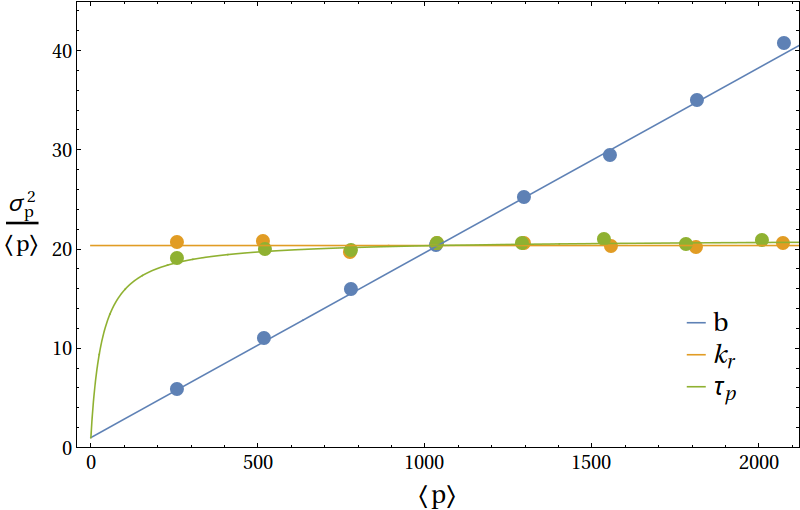
\includegraphics[width=11cm]{mas-sim_simple}
  \caption[Noise in proteins: comparing analytical results and simulations]{\label{fig:mas-sim_simple} Comparison between the results of the simulations (dots) and the analytical results (lines) given by eq. \eqref{eq:noise2}. The Fano factor is plotted vs. the mean. The legend indicates which parameter is varied while the others are fixed.}
\end{figure}

Therefore, the noise and the steady state average can be controlled independently by controlling the burst size $b$. If a cell produces many mRNAs and a few proteins per transcript (small $b$), the noise is reduced. On the contrary, the same average number of proteins can be reached by producing a few mRNAs and many proteins per mRNA (large $b$). In this case the noise is larger. Nevertheless there is an additional factor, reducing noise in this case requires a constant synthesis and degradation of mRNA. This is inefficient for the cells since they are inverting energy in the production of mRNAs from which there will be little proteins translated, representing a disadvantage in fitness. 

This analysis suggests that there is a pay-off between fitness and noise reduction in the cells that has been tuned by evolution according to the necessity of reliability of the particular genetic component. However, we will see that there are other mechanisms, like negative autorregulation, that allow cells to reduce noise in a more efficient way (see sec. \ref{sec:mas-neg_autorreg}).

\section{Several species with linear interactions}

In this section we generalize the previous results to arbitrary genetic network in which the interactions between its components are linear. To introduce the model, consider eqs. \eqref{eq:mas-simple_det_1} and \eqref{eq:mas-simple_det_2}. In matrix notation, they can be written as

\begin{equation}
  \label{eq:matdet}
  \mathbf{\dot{n}} = \left( \mathbf{A} - \mathbf{\Gamma} \right) \mathbf{n},
\end{equation}

where $\mathbf{n}^T=(d,n_1,n_2)$ is the vector of chemical species and the matrices $\mathbf{A}$ and $\mathbf{\Gamma}$ are defined as

\begin{equation*}
  \mathbf{A} =
  \begin{pmatrix}
    0 & 0 & 0 \\
    k_r & 0 & 0 \\
    0 & k_p & 0
  \end{pmatrix},\quad \quad
  \mathbf{\Gamma} =
  \begin{pmatrix}
    0 & 0 & 0 \\
    0 & \gamma_r & 0 \\
    0 & 0 & \gamma_p
  \end{pmatrix}.
\end{equation*}

Hence, $\mathbf{A}$ contains the creation rates and represents how each rate depends on the different species and $\mathbf{\Gamma}$ has the degradation rates, which is diagonal whenever the degradation is not mediated by interactions with other molecules.

Now considering an arbitrary circuit with linear interaction in order that we can write its deterministic equations in the form of eq. \ref{eq:matdet}

Figure \ref{fig:mas-trans_single} and eq. \ref{eq:master} can be generalized according to eq. \ref{eq:matdet} to obtain \ref{fig:mas-trans_many}

\begin{figure}[H]
  \centering
  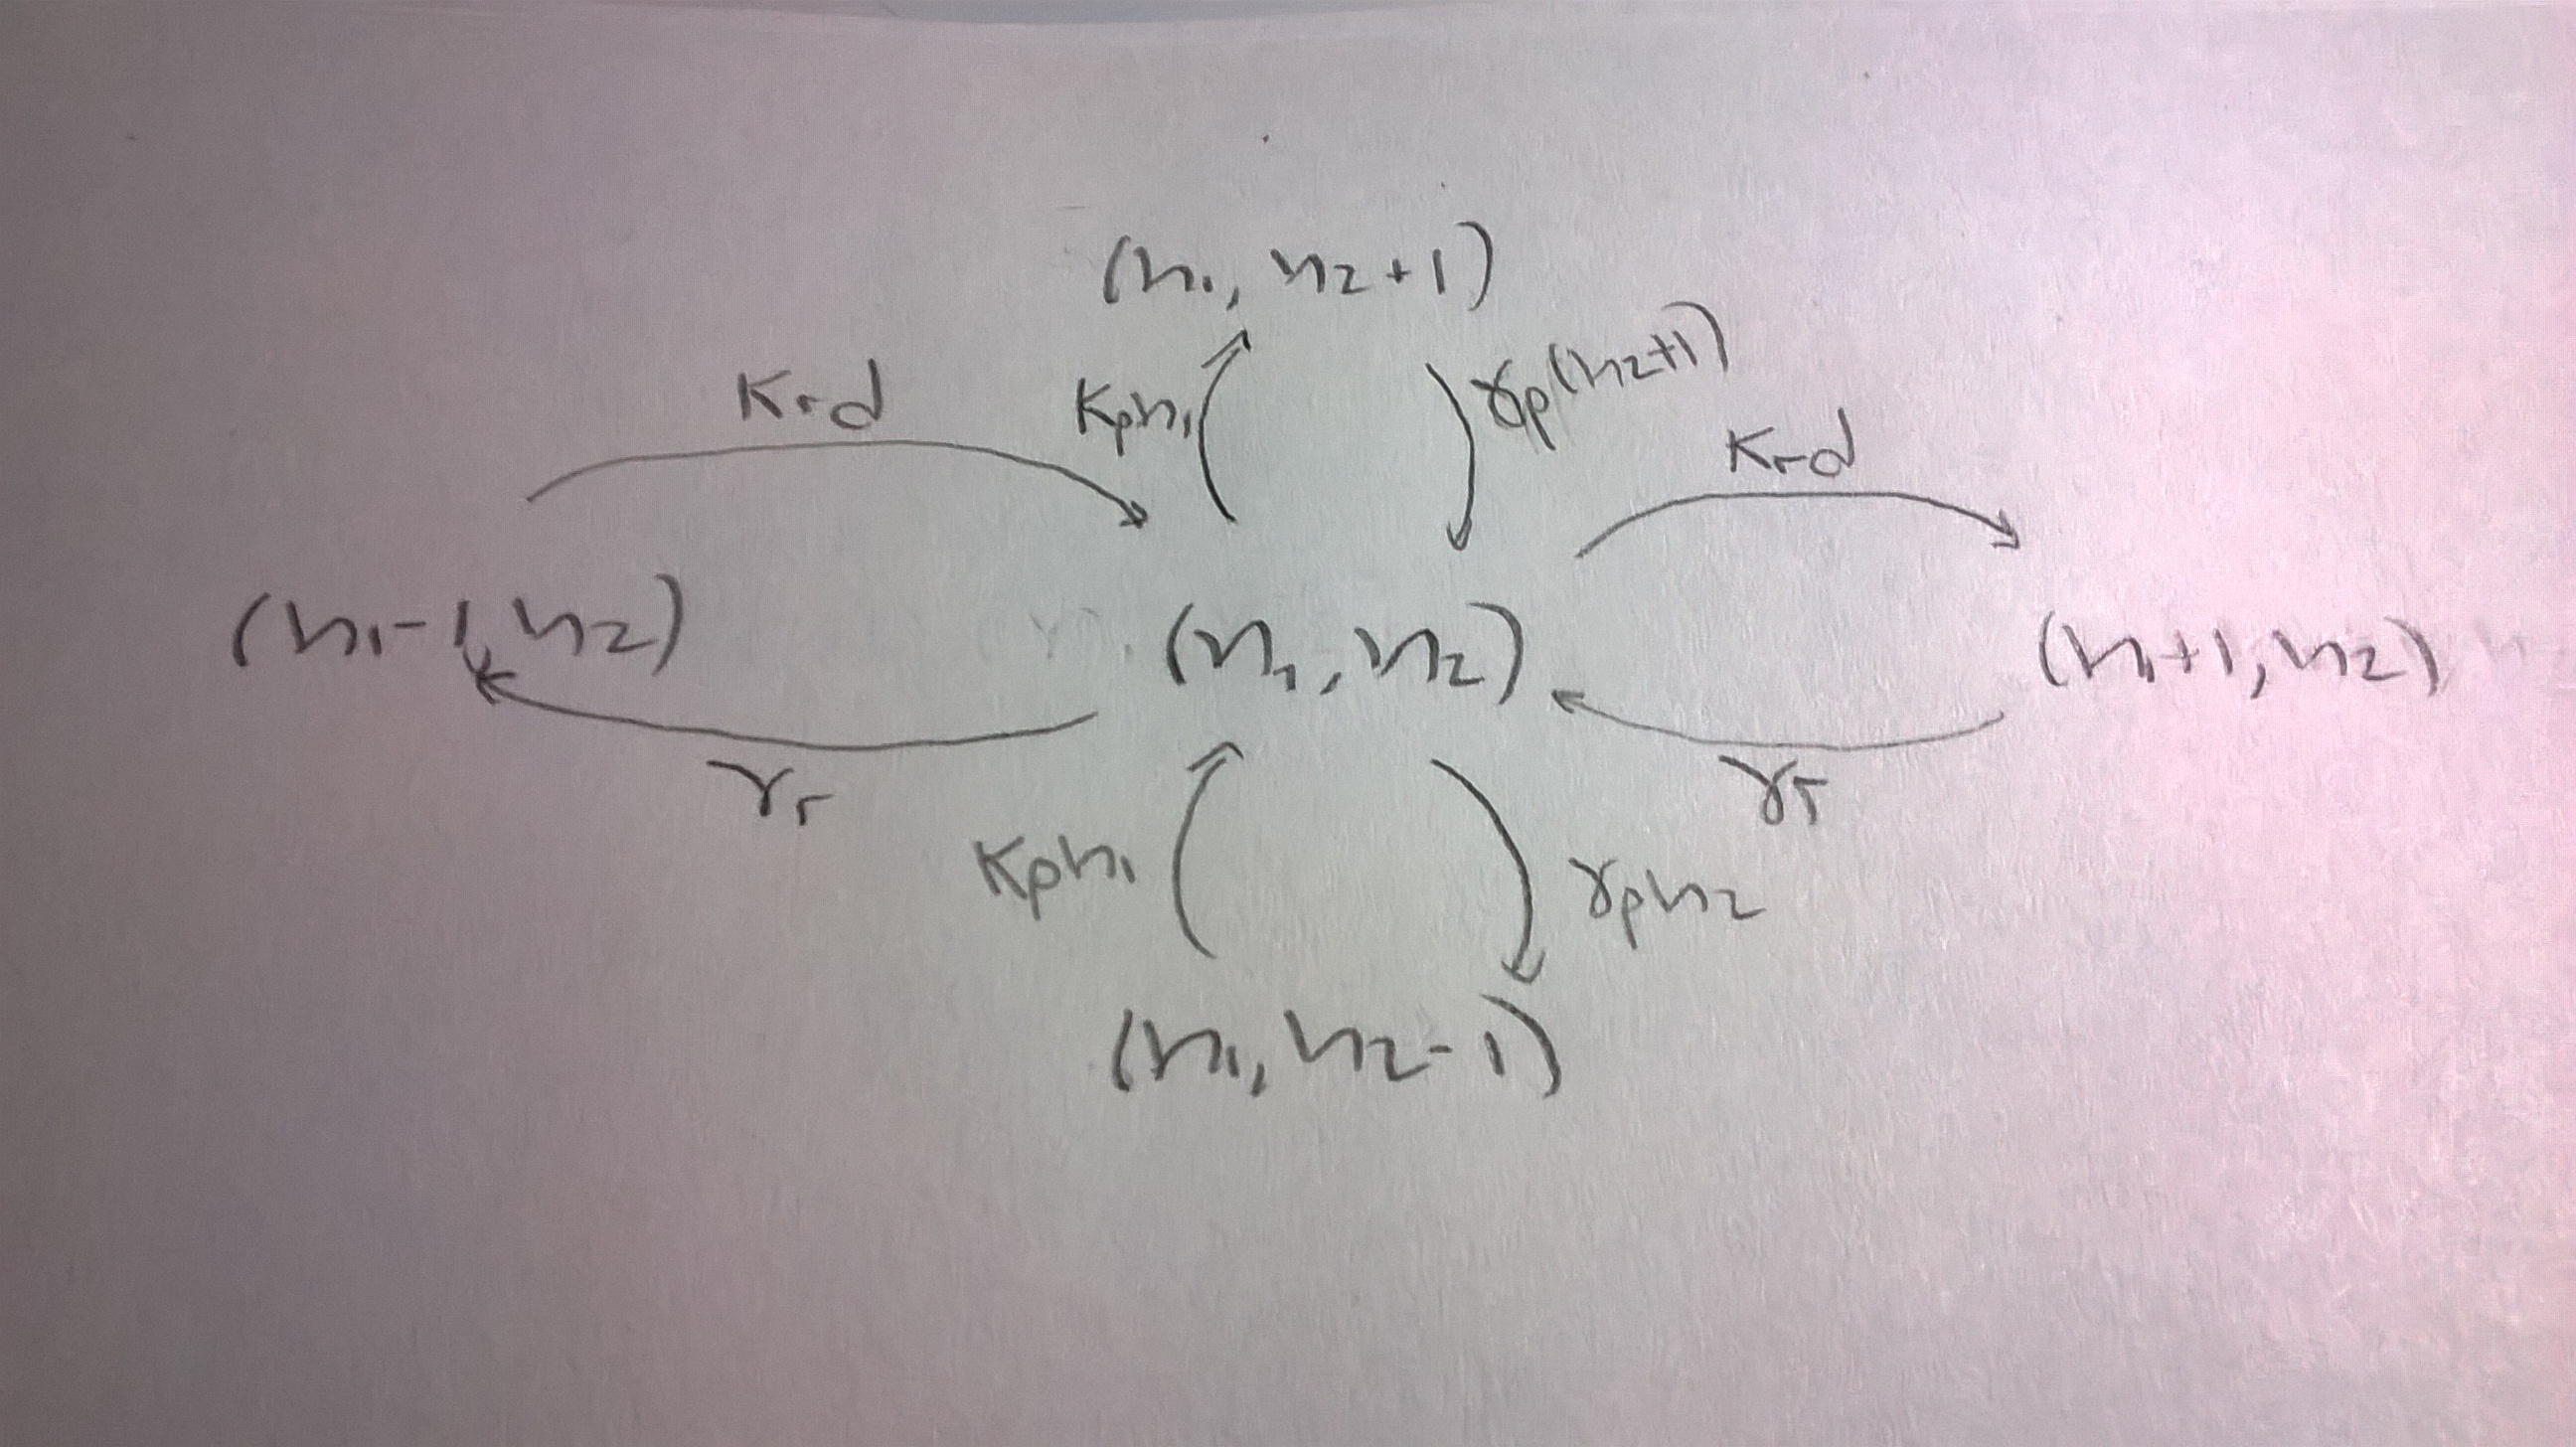
\includegraphics[width=9cm]{mas-trans_many}
  \caption[Transitions between states in general] {\label{fig:mas-trans_many} Scheme of the possible transitions in the case of three species.}
\end{figure}

The master equation can thus be written as (NOTATION, EXPLAIN THE LIMITS OF THE SUM)

\begin{equation}
\label{eq:masterg1}
\dot{f}(n_i) =  \sum_i\left(\sum_j A_{ij}n_j \left( f(n_i-1) - f(n_i) \right) + \sum_j \Gamma_{ij}((n_j+1)f(n_i+1)-n_jf(n_i))\right)
\end{equation}

Decaying is usually dependent on the quantity of the same molecule, assuming this the matrix $\Gamma$ becomes diagonal, i.e. $\Gamma_{ij}=\delta_{ij}\Gamma_j$. With this eq. \ref{eq:masterg1} becomes

\begin{equation}
\label{eq:masterg2}
\dot{f}(n_i) =  \sum_i\left(\sum_j A_{ij}n_j \left( f(n_i-1) - f(n_i) \right) + \Gamma_{i}((n_i+1)f(n_i+1)-n_if(n_i))\right).
\end{equation}

To get an equation for the moment generating functions, we multiply by $z_1^{n_1}\dotsm z_N^{n_N}$ and sum over $n_1,\dotsc n_N$, all from $0$ to $\infty$. For the first term we get an expression like the following (for a fixed $i$) (OJO ABUSE OF NOTATION, SAY LIMITS OF SUM, DEFINE EXPLICITLY ALL Zs?)

\begin{equation}
\label{eq:momg1}
\sum n_j z_1^{n_1}\dotsm z_i^{n_i}\dotsm z_j^{n_j}\dotsm z_N^{n_N} f(n_i) = z_iz_j\sum n_jz_j^{n_j-1}z_i^{n_i}f(n_i) = z_iz_j\frac{\partial F}{\partial z_j}. 
\end{equation} 

Where the same trick done previously on eqs. \ref{eq:mom1} - \ref{eq:mom4} were used. For the second term, similarly to the previous one

\begin{equation}
\label{eq:momg2}
\sum n_jz_j^{n_j}z_i^{n_i}f(n_i) = z_j\frac{\partial F}{\partial z_j}.
\end{equation}

For the third and fourth terms

\begin{equation}
\label{eq:momg3}
\sum (n_i+1)z_i^{n_i}f(n_i+1) = \sum n_i z_i^{n_i-1}f(n_i) = \frac{\partial F}{\partial z_i}.
\end{equation}

\begin{equation}
\label{eq:momg4}
\sum n_iz_i^{n_i}f(n_i) = z_i\frac{\partial F}{\partial z_i}.
\end{equation}

Replacing eqs. \ref{eq:momg1} - \ref{eq:momg4} in eq. \ref{eq:masterg2} we obtain the equation for the moment generating function

\begin{equation}
\dot{F} = \sum_i\left( z_i\sum_jA_{ij}\frac{\partial F}{\partial z_j} - \sum_jA_{ij} z_j \frac{\partial F}{\partial z_j} + \Gamma_i\frac{\partial F}{\partial z_i} - \Gamma_iz_i\frac{\partial F}{\partial z_i}\right),
\end{equation}

which after factoring becomes

\begin{equation}
\label{eq:momg}
\dot{F} = \sum_i (z_i-1)\left(\sum_jA_{ij} z_j \frac{\partial F}{\partial z_j} - \Gamma_i\frac{\partial F}{\partial z_i}\right).
\end{equation}

We have to differentiate it and use the properties (REF) to obtain equations for the moments, differentiating with respect to $z_l$

\begin{equation}
\begin{split}
\frac{\partial \dot{F}}{\partial z_l} &= \sum_i\left[(z_i-1)\left[\sum_jA_{ij}\left(\delta_{jl}\frac{\partial F}{\partial z_j}+z_j\frac{\partial^2 F}{\partial z_j\partial z_l}\right)-\Gamma_i\frac{\partial^2 F}{\partial z_i\partial z_l}\right]\right.\\
&+\left.\delta_{il}\left(\sum_jA_{ij}z_j\frac{\partial F}{\partial z_j}-\Gamma_i\frac{\partial F}{\partial z_i}\right)\right].
\end{split}
\end{equation}

\begin{equation}
\begin{split}
\frac{\partial \dot{F}}{\partial z_l} &= \sum_i(z_i-1)\left[A_{il}\frac{\partial F}{\partial z_l}+\sum_jA_{ij}z_j\frac{\partial^2 F}{\partial z_j\partial z_l}-\Gamma_i\frac{\partial^2 F}{\partial z_i\partial z_l}\right]\\
&+\sum_jA_{lj}z_j\frac{\partial F}{\partial z_j}-\Gamma_l\frac{\partial F}{\partial z_l}.
\end{split}
\end{equation}

Evaluando en $z_i=0$ para todo $i=1,\dotsc,N$ obtenemos usando las propiedades (CITAR)

\begin{equation}
\dot{\langle n_l \rangle} = \sum_jA_{lj}\langle n_j\rangle-\Gamma_l\langle n_l\rangle.
\end{equation}

Which can be written in matrix form

\begin{equation}
\dot{\langle \mathbf{n}\rangle} = (\mathbf{A}-\mathbf{\Gamma})\langle \mathbf{n}\rangle.
\end{equation}

Which is the same as  eq. (REF), as expected. Now differentiating again with respect to $z_m$ and some algebra

\begin{equation}
\begin{split}
\frac{\partial^2 \dot{F}}{\partial z_l \partial z_m} &= \sum_i(z_i-1) \left(A_{im}\frac{\partial^2F}{\partial z_i \partial z_m} + \sum_jA_{ij}z_j\frac{\partial^3F}{\partial z_j \partial z_l \partial z_m}+A_{il}\frac{\partial^2F}{\partial z_l\partial z_m} - \Gamma_i\frac{\partial^3F}{\partial z_i \partial z_l \partial z_m}   \right)\\
&+\sum_jA_{mj}z_j\frac{\partial^2F}{\partial z_j\partial z_l}+A_{ml}\frac{\partial F}{\partial z_l} - \Gamma_m\frac{\partial^2F}{\partial z_l\partial z_m} + A_{lm}\frac{\partial F}{\partial z_m} + \sum_jA_{lj}z_j\frac{\partial^2F}{\partial z_j\partial z_m}-\Gamma_l\frac{\partial^2F}{\partial z_l\partial z_m}.
\end{split}
\end{equation}

Evaluating at $z_i=1$ for all $i$ we obtain

\begin{equation}
\frac{\partial^2\dot{F}}{\partial z_l \partial z_m} = \sum_jA_{mj}z_j\frac{\partial^2F}{\partial z_j\partial z_l}+A_{ml}\frac{\partial F}{\partial z_l} - \Gamma_m\frac{\partial^2F}{\partial z_l\partial z_m} + A_{lm}\frac{\partial F}{\partial z_m} + \sum_jA_{lj}z_j\frac{\partial^2F}{\partial z_j\partial z_m}-\Gamma_l\frac{\partial^2F}{\partial z_l\partial z_m}.
\end{equation}

Which can be rewritten as

\begin{equation}
  \begin{split}
    \frac{\partial^2\dot{F}}{\partial z_l \partial z_m} &= \sum_j\left(A_{mj}z_j-\Gamma_{mj}\right)\frac{\partial^2F}{\partial z_j\partial z_l} + \sum_jA_{mj}\delta_{jl}\frac{\partial F}{\partial z_j}\\
&+\sum_j\left(A_{lj}z_j-\Gamma_{lj}\right)\frac{\partial^2F}{\partial z_j\partial z_m} + \sum_jA_{lj}\delta_{jm}\frac{\partial F}{\partial z_j}.
  \end{split}
\end{equation}

Which is valid for all $l$ and $m$, evaluating at $z_i=1$ for all $i$ we get in matrix form

%\frac{\partial^2F}{\partial z_l \partial z_m}

\begin{equation}
  \boxed{\nabla\nabla^T\dot{F}|_1 = \left(\left(\mathbf{\Gamma} - \mathbf{A}\right)\nabla\nabla^TF|_1 - \mathbf{A}\mathbf{\Theta} F|_1\right)+\left(\left(\mathbf{\Gamma} - \mathbf{A}\right)\nabla\nabla^TF|_1 - \mathbf{A}\mathbf{\Theta} F|_1\right)^T}
\end{equation}

Where $\Theta_{ij} \coloneqq \delta_{ij}\frac{\partial}{\partial z_i}$. The set of linear equations can be solved for the moments and correlation using a computer program.

\section{Several species with non-linear interactions - Negative autorregulation}
\label{sec:mas-neg_autorreg}

\begin{figure}[H]
  \centering
  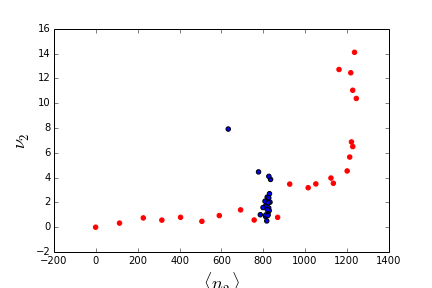
\includegraphics[width=9cm]{mas-sim_autorreg}
  \caption[Autorregulation simulation results]{\label{fig:mas-sim_autorreg} Simulation for the case of autorregulation}
\end{figure}

\chapter{The Fluctuation-Dissipation theorem (FDT)}

This chapter is based on the work of J. Paulsson in \cite{paulsson04} and \cite{paulsson05}

\todo[inline]{Do this chapter}

\section{Statement of the FDT}

\section{Example: simple gene}

\section{The logarithmic gain}
\label{sec:log_gain}

\chapter{Cascade of regulation - The Langevin equation}

\section{Intrinsic noise in a single gene using the Langevin approach}

In the Langevin approach, a term representing the noise of the system is added to the deterministic equations instead of considering the transition rates between states explicitely. Knowing some of the statistical properties of the noise term will allow us to find the noise in the number of species. In this section we will use the Langevin approach to find the intrinsic noise for a single gene.

Consider the model used on section \ref{sec:mas-single_gene}. For each of the deterministic equations (eqs. \label{eq:mas-simple_det_1} and \label{eq:mas-simple_det_2}), a stochastic process is added that accounts for the intrinsic noise. Including the terms $\mu_1(t)$ and $\mu_2(t)$ results in

\begin{align}
  \dot{n_1}(t) &= k_rd-\gamma_rn_1(t) + \mu_1(t)\label{eq:lan-simple_1},\\
  \dot{n_2}(t) &= k_pn_1(t)-\gamma_pn_2(t) + \mu_2(t)\label{eq:lan-simple_2}.
\end{align}

Now $n_1(t)$ and $n_2(t)$ are stochastic processes. We need to have some information of the noise terms in order to proceed. First, as we saw in chapter \ref{ch:master}, the averages must follow the deterministic behavior. By taking averages on both sides of eqs. \label{eq:lan-simple_1} - \label{eq:lan-simple_2} and imposing this condition we get

\begin{equation*}
  \langle\mu_r\rangle(t) = \langle\mu_r\rangle(t) = 0.
\end{equation*}

Also, assuming white noise statistics, the autocorrelations are given by

\begin{align}
  \langle\mu_1(t)\mu_1(t+\tau)\rangle &= q_1\delta(\tau),\label{eq:lan-simple_cor1} \\
  \langle\mu_2(t)\mu_2(t+\tau)\rangle &= q_2\delta(\tau). \label{eq:lan-simple_cor2}
\end{align}

This means that we will assume that there is no correlation between the values of the noise term at different times. The coefficients $q_1$ and $q_2$ determine the strenght of the noise and will be treated later. Also, the intrinsic noise must be fully uncorrelated among mRNA and proteins, hence

\begin{equation}
  \langle\mu_1(t)\mu_2(t+\tau)\rangle = 0. \label{eq:lan-simple_cor12}
\end{equation}

We will use eqs. \eqref{eq:lan-simple_cor1} - \eqref{eq:lan-simple_cor12} to find the noise in mRNA and protein numbers. Define the difference with respect to steady state average as $\delta n_1$ and $\delta n_2$, i.e. $\delta n_i \coloneqq n_i - \langle n_i\rangle_s$, for $i=1,2$. In terms of these quantities the eqs. become

\begin{align}
  \dot{\delta n_1}(t) &= -\gamma_r\delta n_1(t) + \mu_1(t)\label{eq:lan-simple_d1},\\
  \dot{\delta n_2}(t) &= k_p\delta n_1(t) -\gamma_p\delta n_2(t) + \mu_2(t)\label{eq:lan-simple_d2}.
\end{align}

Fourier transforming and using the fact that $\left[\mathscr{F}(\dot{x}(t))\right](\omega) = i\omega \hat{x}$, where $\hat{x}\coloneqq\mathscr{F}(x)$ we get 

\begin{equation}
  \delta\hat{n}_1(\omega) = \frac{\hat{\mu}_1(\omega)}{\gamma_r+i\omega},\quad\quad \delta\hat{n}_2(\omega) = \frac{\delta\hat{n}_1(\omega) + \hat{\mu}_2(\omega)}{\gamma_p+i\omega}.
\end{equation}

Taking the average of the square norm of the first expression we obtain the power spectrum for $\delta n_1$

\begin{equation*}
  \langle|\delta\hat{n}_1|^2\rangle = \frac{\langle|\hat{\mu}_1|^2\rangle}{\omega^2+\gamma^2} = \frac{q_1}{\omega^2+\gamma_r^2},
\end{equation*}

because by using the Wiener-Khinchin theorem (eq. \eqref{eq:con-wkth}) and eq. \eqref{eq:lan-simple_cor1} we obtain $\langle|\hat{\mu}_1|^2\rangle = q_1^2$. Making the inverse Fourier transform and evaluating at $t=0$ yields the variance of $n_1$

\begin{equation*}
  \sigma^2(n_1) = \langle\delta n_1^2\rangle = q_1^2 \left[\mathscr{F}^{-1}\frac{1}{\omega^2+\gamma_r^2}\right](t=0) = q_1^2\int_{-\infty}^\infty\frac{1}{\omega^2+\gamma_r^2}\frac{\mathrm{d}\omega}{2\pi} = \frac{q_1^2}{2\gamma_r}.
\end{equation*}

The integral can be easily solved in the complex plane or by trigonometric substitution. Keeping in mind that mRNA creation and destruction are single step Poisson processes and as we saw on chapter \ref{ch:master}, the variance must be equal to the average. Imposing this condition, we find that $q_1$ is given by

\begin{equation*}
  q_1^2 = 2\gamma_r\sigma^2(n_1) = 2\gamma_r\langle n_1\rangle = 2k_rd
\end{equation*}

There is a more general procedure for finding the noise strenght $q$ in steady state. It can be shown that for single step Poisson processes it is given by the square root of the sum of the rates for all the events evaluated at the steady state average. If amount $x$ of some molecule follows the deterministic equation

\begin{equation*}
  \dot{x} = f(x) - g(x),
\end{equation*}

then

\begin{equation*}
  q_x = \sqrt{f(\langle x\rangle_s)+g(\langle x\rangle_s)}
\end{equation*}



\todo[inline]{Prove this!?}

\section{Model circuit for the cascade}
The calculations shown in this chapter are based in the work of J. M. Pedraza and A. van Oudenaarden \cite{pedraza05}. They build the model circuit and tested the theoretical results experimentally. 

\todo[inline]{Cite Juan M. PhD thesis}

We will consider a set of genes whose interactions are shown on figure \ref{fig:lan-circuit} considering both intrinsic and extrinsic sources of noise. The intrinsic part refers to the inherent noise due to the low number of molecules and the nature of the reactions. This was the only source of noise consider on the previous chapter. The extrinsic part arises from another factors, such as environmental fluctuations or variations in intracellular concentrations due to sudden changes on cell volume. These factors causes fluctuations in every component of the cell and thus extrinsic noise is correlated among the different genes, while intrinsic noise is not \cite{elowitz02}.

\todo[inline]{Explain intrinsic/extrinsic noise in a section on concepts.}
\todo[inline]{Explain plasmid and chromosomal DNA, and constitutive promoter.}

Fig. \ref{fig:lan-circuit} shows a genetic circuit built from four genes to be used on bacteria. Gene $0$ is located in the chromosome while genes $1$ to $3$ are located in plasmids, hence, their expression is subjected to noise caused by plasmid number fluctuations. Genes $0$ codifies for \textit{LacI} and $3$ for the red fluorescent protein \textit{rfp}. Both are regulated by a constitutive promoter, gene $1$ has the promoter P$_\text{lac}$, which regulates the expression of \textit{tetR} and \text{cfp} (cyan fluorescent protein). The transcription from P$_\text{lac}$ is repressed by \textit{LacI}. Also, the repressing effect of \textit{LacI} is inhibited by IPTG.

\begin{figure}[H]
  \centering
  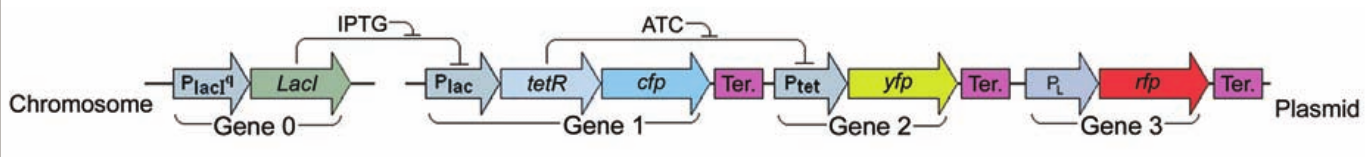
\includegraphics[width=15cm]{lan-circuit}
  \caption[Circuit used for the Langevin model]{\label{fig:lan-circuit} Circuit used in the Langevin model (from \cite{pedraza05}).}
\end{figure}

A similar effect happens on gene $2$, the tetracycline promoter P$_\text{tet}$, which regulated the expression of the yellow fluorescent protein \textit{yfp}. It is repressed by \textit{tetR} and the repressing effect of \textit{tetR} is also inhibited by ATC.

Therefore, both IPTG and ATC are environmental signals that are used to regulate the coupling between the different genes of the cascade. Notice that for instance, at higher quantities of IPTG, expression of gene $1$ is low since the repression over it is reduced. This also causes that without ATC, the expression of gene $2$ is high. 

The fluorescent proteins are used to quantify experimentally via fluorescence microscopy the expressions of each gene, which will be proportional to the intensity of the flourescence on each color. \textit{tetR} and \textit{cfp} are transcribed bicistronically in order to be able to quantify \textit{tetR} levels. We will assume that protein degradation is caused only by cell division (i.e. there is no active degradation). That allow us to use the same degradation constant for all proteins, and in particular, to assume that the behavior of \textit{cfp} reproduces exactly the behavior of \textit{tetR}. 

We will label the concentrations of \textit{LacI}, \textit{tetR} (and \textit{cfp}), \textit{yfp} and \textit{rfp} as $x_0$, $x_1$, $x_2$, and $x_3$, respectively.

\section{Mathematical derivations}

The differential equation for the mRNA will not be considered, we will write the equation for the proteins and include the effect of mRNA in the rate of creation $k$. The results of the previous chapter for the noise in proteins caused by mRNA will also be considered. The deterministic equation for the concentration of proteins of gene $0$ is 

\begin{equation}
\label{eq:detgene0}
\dot{x_0}(t) = k - \gamma x_0(t).
\end{equation}

Where now $k$ represents the average number of proteins created per unit time.\footnote{For a better understanding of this point. If we assume $\gamma_r\ll\gamma_p$, we can treat the mRNA in steady state, hence eq. \eqref{eq:mas-simple_det_2} becomes eq. \eqref{eq:detgene0} with $k \coloneqq k_p\langle n_1\rangle_s =  \frac{k_pk_r}{\gamma_r} = k_rb$.}In the Langevin approach noise terms are added to the previous equation representing the intrinsic noise $\mu_0(t)$ and the global noise $\xi_0(t)$. Hence, the equation for the stochastic process $x_0(t)$ is

\begin{equation}
\label{eq:gene0}
\dot{x_0}(t) = k - \gamma x_0(t) + \mu_0(t) + \xi_0(t).
\end{equation}

To find the correlations and the coefficient of variation, we need some information about the noise terms. First, the average of proteins $\langle x_0 \rangle (t)$ should follow the deterministic equation \eqref{eq:detgene0}, therefore

\begin{equation*}
\langle\mu_0\rangle(t) = \langle\xi_0\rangle(t) = 0.
\end{equation*}

Second, we will assume white noise statistics for both sources, that is, the values of the noise terms at different times are uncorrelated. Then

\begin{align}
\langle\mu_0(t)\mu_0(t+\tau)\rangle&=2\gamma(b_0+1)\bar{x}_0\delta(\tau),\label{eq:corin0}\\
\langle\xi_0(t)\xi_0(t+\tau)\rangle&=2\gamma\eta_G^2\bar{x}_0^2\delta(\tau). \label{eq:corex0}
\end{align}

\todo[inline]{Understand and explain more the constants and the assumption of white noise}

where $\eta_G$ is the strenght of the global noise, a parameter that is measured experimentally, and $b_0$ is the average number of protein produced per mRNA. In this section the bar denotes steady state average. Also, since both sources of noise are uncorrelated

\begin{equation}
\label{eq:corinex0}
\langle\mu_0(t)\xi_0(t+\tau)\rangle = 0.
\end{equation}

Define $\delta x_0 \coloneqq x_0 - \bar{x}_0$, replacing this on eq. \eqref{eq:gene0} we get

\begin{equation}
\frac{\mathrm{d}}{\mathrm{d}t}\left(\delta x_0(t) + \bar{x}_0\right) = k - \gamma (\delta x_0(t) + \bar{x}_0) + \mu_0(t) + \xi_0(t),
\end{equation}

Using the fact that $\bar{x}_0=k/\gamma$ we get

\begin{equation}
\label{eq:dgene0}
\dot{\delta x_0}(t) = -\gamma \delta x_0(t) + \mu_0(t) + \xi_0(t).
\end{equation}

We will Fourier transform the equation, find its square norm and use the Wiener-Khinchin theorem (eq. \eqref{eq:con-wkth}) to find the autocorrelations in terms of the power spectrum and to write the power spectrum of $\mu(t)$ and $\xi(t)$ in terms of their autocorrelations.

Taking the Fourier transform of eq. \eqref{eq:dgene0} and recalling that $[\mathscr{F}(\frac{\mathrm{d}x(t)}{\mathrm{d}t})](\omega) = i\omega \mathscr{F}(x(t))(\omega)$ for a function of time $x(t)$, we obtain after solving for $\hat{\delta x_0}$

\begin{equation}
\label{eq:fgene0}
\hat{\delta x_0}(\omega) = \frac{\hat{\mu_0}+\hat{\xi_0}}{\gamma + i\omega}.
\end{equation}

Taking the square norm and averaging we get

\begin{equation}
\left\langle |\hat{\delta x_0}|^2 \right\rangle = \frac{\left\langle|\hat{\mu_0}|^2\right\rangle + \left\langle\hat{\mu_0}^*\hat{\xi_0}\right\rangle+\left\langle\hat{\mu_0}\hat{\xi_0}^*\right\rangle+\left\langle|\hat{\xi_0}|^2\right\rangle}{\gamma^2 + \omega^2},
\end{equation}

And using the Wiener-Khinchin theorem and eqs. \eqref{eq:corin0} - \eqref{eq:corinex0}

\todo[inline]{Explain with more detail here}

\begin{equation}
  \label{eq:pgene0}
  \begin{split}
    \left\langle |\hat{\delta x_0}|^2 \right\rangle &= \frac{\left(2\gamma(b_0+1)\bar{x_0}+ 2\gamma\eta_G^2\bar{x_0}^2\right)\mathscr{F}(\delta(t))}{\gamma^2+\omega^2}\\
    &=\frac{2\gamma\bar{x_0}^2\left(\nicefrac{(b_0+1)}{\bar{x_0}}+ \eta_G^2\right)}{\gamma^2+\omega^2},
  \end{split}
\end{equation}

where the cross terms are zero by eq. \eqref{eq:corinex0}. Applying the inverse Fourier transform at $t=0$ we get

\begin{equation*}
\langle \delta x_0^2 \rangle = 2\gamma\bar{x_0}^2\left(\nicefrac{(b_0+1)}{\bar{x_0}}+ \eta_G^2\right)\frac{1}{2\pi}\int_{-\infty}^{\infty}\frac{d\omega}{\omega^2+\gamma^2}
\end{equation*}

The integral can be easily solved by residues resulting in $\pi/\gamma$, therefore

\begin{equation*}
\langle \delta x_0^2 \rangle = \bar{x_0}^2\left(\frac{(b_0+1)}{\bar{x_0}}+ \eta_G^2\right)
\end{equation*}

And dividing by $\bar{x_0}^2$, we obtain the coefficient of variation

\begin{equation}
  \label{eq:etagene0}
  \boxed{\eta_0^2 = \frac{(b_0+1)}{\bar{x_0}}+ \eta_G^2 = \eta_{0\text{int}}^2+\eta_G^2}.
\end{equation}

This approach enabled us to explicitly separate the total noise of gene $0$ in the intrinsic and the extrinsic part. Now we will make the calculation for gene $1$, which follows the equation.

\begin{equation}
\label{eq:gene1}
\dot{x_1}(t) = k_1(x_{0A})-\gamma x_1+\mu_1+\xi_1
\end{equation}

The decay rate $\gamma$ is the same for gene $1$ than for gene $0$ after making the assumption that the decay depends only on dilution due to cellular growth. The creation rate $k_1$ is a Hill equation for activation. The statistics for the noise terms are analogous to eqs. \eqref{eq:corin0} - \eqref{eq:corinex0}. We also need to know in this case the correlations between the noise terms corresponding to gene $0$ and the ones corresponding to gene $1$. As we have said, extrinsic sources of noise are uncorrelated

\todo[inline]{Explain more about the dilution, perhaps before}

\begin{equation}
\label{eq:corcross01}
\langle\mu_0(t)\mu_1(t+\tau)\rangle = \langle\mu_0(t)\xi_1(t+\tau)\rangle = \langle\mu_1(t)\xi_0(t+\tau)\rangle = 0,
\end{equation}

but the extrinsic parts of the noise of genes $0$ and $1$ are correlated. In analogy with eq. \eqref{eq:corex0} we get

\begin{equation}
  \langle\xi_0(t)\xi_1(t+\tau)\rangle = 2\gamma\eta_G^2\bar{x_0}\bar{x_1}\delta(\tau).
\end{equation}

\todo[inline]{Also, understand and explain the q term here}

We proceed in a similar way to gene $0$. Defining $\delta x_1(t) \coloneqq x_1(t) - \bar{x_1}$, writing eq. \eqref{eq:gene1} in terms of $\delta x_1$, $\delta x_{0A}$, and making a Taylor expansion of $f_1$ to first order in $x_{0A}$ about $\bar{x}_{0A}$ we obtain.

\begin{equation}
\dot{\delta x_1} = k_1(\bar{x_{0A}}) + \left.\frac{dk_1(x_{0A})}{dx_{0A}}\right|_{\bar{x_{0A}}}\delta x_{0A} - \gamma(\delta x_1 + \bar{x_1}) + \mu_1 + \xi_1,
\end{equation}

but from eq. \eqref{eq:gene1} we can see that $\bar{x_1} = \nicefrac{k_1(\bar{x_{0A}})}{\gamma}$, therefore

\begin{equation}
  \label{eq:dgene1}
  \dot{\delta{x_1}(t)}=c_1\delta x_{0A}-\gamma\delta x_1 + \mu_1 \xi_1,
\end{equation}

where $c_1 \coloneqq \left.\nicefrac{dk_1(x_{0A})}{dx_{0A}}\right|_{\bar{x_{0A}}}$ Fourier transforming and solving for $\hat{\delta x_1}$ we get

\begin{equation*}
  \hat{\delta x_1}=\frac{c_1\hat{\delta x_{0A}}+\hat{\mu_1}+\hat{\xi_1}}{\gamma + i\omega}.
\end{equation*}

Taking the square norm and averaging

\begin{equation*}
  \label{eq:pgene1}
  \begin{split}
    \left\langle|\hat{\delta x_1}|^2\right\rangle &= \frac{1}{\omega^2+\gamma^2}\left(c_1\hat{\delta x_{0A}} + \hat{\mu_1} + \hat{\xi_1}\right)\left(c_1\hat{\delta x_{0A}}^* + \hat{\mu_1}^* + \hat{\xi_1}^*\right)\\
    &=\frac{1}{\omega^2+\gamma^2}\left(c_1^2 \left\langle|\hat{\delta x_{0A}}|^2\right\rangle + c_1\left(\langle\hat{\delta x_{0A}}\hat{\xi_1}^*\rangle+\langle\hat{\delta x_{0A}}^*\hat{\xi_1}\rangle\right) +  \left\langle|\hat{\mu_1}|^2\right\rangle +  \left\langle|\hat{\xi_1}|^2\right\rangle\right)
  \end{split}
\end{equation*}

Using the Wiener-Khinchin theorem and the equations for the correlations we get

\begin{align*}
  \left\langle|\hat{\mu_1}|^2\right\rangle &= 2\gamma(b_1+1)\bar{x_1},\\
  \left\langle|\hat{\xi_1}|^2\right\rangle &= 2\gamma\eta_G^2\bar{x_1}^2,
\end{align*}

since the Fourier transform of the Dirac delta is $1$. Also, from eqs. \eqref{eq:fgene0} and \eqref{eq:pgene0} we get

\begin{align*}
\left\langle|\hat{\delta x_{0A}}|^2\right\rangle &= \frac{2\gamma\bar{x_0}^2\left(\nicefrac{(b_0+1)}{\bar{x_0}}+ \eta_G^2\right)}{\gamma^2+\omega^2},\\
\langle\hat{\delta x_{0A}}\hat{\xi_1}^*\rangle &= \frac{1}{\gamma+i\omega}\left(\langle\hat{\mu_0}\hat{\xi_1}^*\rangle + \langle\hat{\xi_0}\hat{\xi_1}^*\rangle \right) = \frac{\langle\hat{\xi_0}\hat{\xi_1}^*\rangle}{\gamma+i\omega}\\
\langle\hat{\delta x_{0A}}^*\hat{\xi_1}\rangle &= \frac{1}{\gamma-i\omega}\left(\langle\hat{\mu_0}^*\hat{\xi_1}\rangle + \langle\hat{\xi_0}^*\hat{\xi_1}^*\rangle \right) = \frac{\langle\hat{\xi_0}^*\hat{\xi_1}\rangle}{\gamma-i\omega}
\end{align*}

Where the last step in the last two equations comes from the Wiener-Khinchin theorem and eq. \eqref{eq:corcross01}. Replacing the previous equations in eq. \eqref{eq:pgene1} and taking the inverse transform we get for the variance

\begin{equation}
  \begin{split}
    \langle \delta x_1^2\rangle &= 2\gamma\bar{x_0}^2c_1^2\left(\nicefrac{(b_0+1)}{\bar{x_0}}+ \eta_G^2\right)\frac{1}{2\pi}\int_{-\infty}^{\infty}\frac{d\omega}{(\omega^2+\gamma^2)^2}\\
    &+2\gamma\eta_G^2\bar{x_0}\bar{x_1}c_1\frac{1}{2\pi}\left(\int_{-\infty}^{\infty}\frac{d\omega}{(\gamma + i\omega)(\omega^2+\gamma^2)} + \int_{-\infty}^{\infty}\frac{d\omega}{(\gamma - i\omega)(\omega^2+\gamma^2)}\right)\\
    &+2\gamma\bar{x_1}^2 \left(\nicefrac{(b_1+1)}{\bar{x_1}}+\eta_G^2\right)\frac{1}{2\pi}\int_{-\infty}^{\infty}\frac{d\omega}{\omega^2+\gamma^2}.
  \end{split}
\end{equation} 

Solving the integrals in the complex plane and rearranging

\begin{equation}
  \langle \delta x_1^2\rangle = \frac{c_1^2\bar{x_0}^2}{2\gamma^2}\left(\nicefrac{(b_0+1)}{\bar{x_0}}+ \eta_G^2\right) + \frac{c_1\eta_G^2\bar{x_0}\bar{x_1}}{\gamma} + \bar{x_1}^2\left(\nicefrac{(b_1+1)}{\bar{x_1}}+\eta_G^2\right).
\end{equation}

Writing in terms of the logarithmic gain $H_{ji}\coloneqq -\frac{\langle x_i\rangle}{\langle x_j\rangle}\frac{1}{\gamma_j}\frac{\mathrm{d} f_j(x_i)}{\mathrm{d}x_i}$, in this case it becomes $H_{10}=-\frac{c_1\bar{x_0}}{\gamma x_1}$. Dividing by $\bar{x_1}^2$ and rearranging

\begin{equation}
  \label{eq:etagene1}
  \boxed{\eta_1^2 = \eta_{1\text{int}}^2 + \frac{1}{2}H_{10}^2\eta_0^2+\eta_G^2\left(1-H_{10}\right)}.
\end{equation}

\todo[inline]{TODO: Explain a lot more about the logarithmic gain}

Where $\eta_{1\text{int}}^2 = \nicefrac{(b_1+1)}{\bar{x_1}}$ and $\eta_0^2$ is given by eq. \ref{eq:etagene0}.

The result can be interpreted as follows, the total noise in gene one is given by the intrinsic part, the noise from gene $0$ that is propagated to gene $1$ (including both its intrinsic and global part) and the global noise that enters directly into gene $1$. The factor of $1/2$ arises from the time averaging since we assumed equal degradation rates for both proteins.

\todo[inline]{See if it is better to do it with different gammas}

For gene $2$ we proceed similarly, with analogous statistics for the noise terms, the resulting noise is

\begin{equation}
  \label{eq:etagene2}
  \boxed{\eta_2^2 = \eta_{2\text{int}}^2 + \frac{1}{2}H_{21}^2\eta_1^2+\frac{1}{8}H_{21}^2H_{10}^2\eta_0^2+\eta_G^2\left(1-H_{21}-\frac{1}{4}H_{21}^2H_{10}+\frac{1}{2}H_{21}H_{10}\right)}.
\end{equation}

Which contains the intrinsic noise of gene $2$, the contribution from the total noise of gene $1$, the contribution from the total noise of gene $0$ that is transmitted first to gene $1$ and then to gene $2$ and the global noise that enters directly. 

The correlations can be found in a similar fashion.

\todo[inline]{TODO: Find the correlations and do the analysis that JM did on SysBio class}

\section{Explicit expressions for the logarithmic gain}



\section{Analysis and implications}

As it can be noticed in eqs. \eqref{eq:etagene0}, \eqref{eq:etagene1} and \eqref{eq:etagene2}, the noise propagation follows the sequence of fig. \ref{fig:lan-noise_sources}. For each gene there is an independent intrinsic noise a correlated global noise, and both the transmitted global and intrinsic noise between the genes of the cascade whose strenght is determined by the logarithmic gain $H$.

\begin{figure}[H]
  \centering
  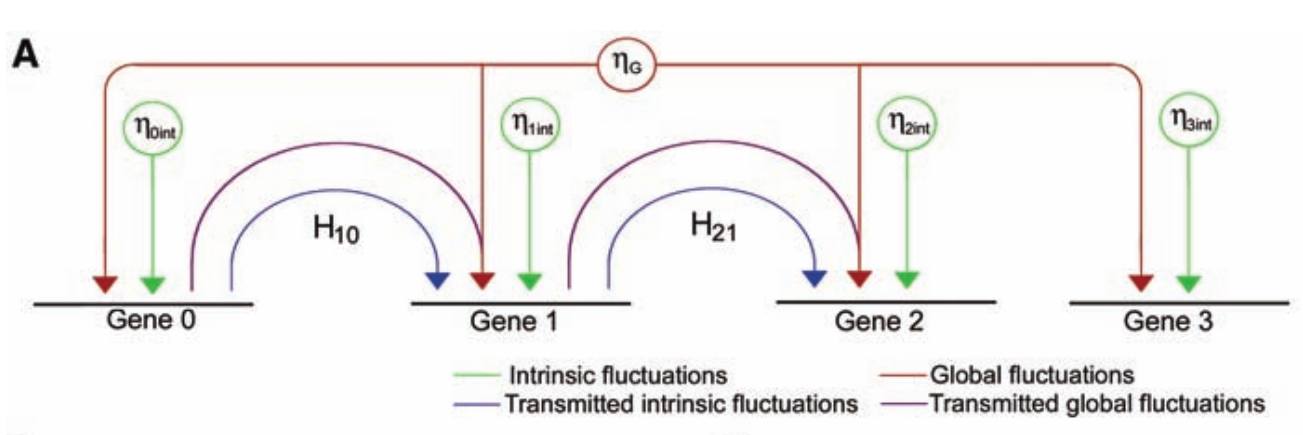
\includegraphics[width=15cm]{lan-noise_sources}
  \caption[Propagation of noise through a cascade]{\label{fig:lan-noise_sources} Different sources of noise and their propagation along the cascade of regulation (from \cite{pedraza05}).}
\end{figure}

\todo[inline]{TODO: Analyze the results physically (recall SysBio class), reproduce the graphics and analyze them}

This approach enables us to calculate the coefficient of variation for a cascade of regulation and separate the different sources of noise. Also, it enables to write the effect of the upstream genes in terms of the logarithmic gain, making it very intuitive. The results of the theoretical model were tested with experiments where the genes that are part of the cascade are transcribed bicistronicaly with fluorescent reporters. The fluctuations in the intensity of the reporters was used to measure the noise in the population of cells.

\chapter{Effects of bursting and senescence}
\label{ch:bursting}

In the previous chapters we have modeled some genetic circuits that satisfy the simple assumptions of a single step Poisson process. These include the creation and degradation of mRNA molecules and proteins in single steps with times between events that are memoryless. Nevertheless, there exist many different gene expression and regulation mechanisms affecting many genetic systems, mostly in eukaryotic cells. 

For instance, there may be cases of bursting in synthesis. This occurs when several molecules produced per creation events, and both the time between events and the number of molecules produced in an event is a random number following some arbitrary distribution (fig. \ref{fig:bur-examples} - left). On the other hand, some molecules can senesce before being completely degraded. That is, they transit over several steps in their process of degradation (fig. \ref{fig:bur-examples} - right). To model these phenomena, it is not enough to assume single step Poisson processes. In this chapter we will use the FDT and elements of basic probability to analyze the effect of bursting and senescence on noise.

This chapter is based on the work done by J. M. Pedraza and J. Paulsson in \cite{pedraza08}.

\begin{figure}[H]
  \centering
  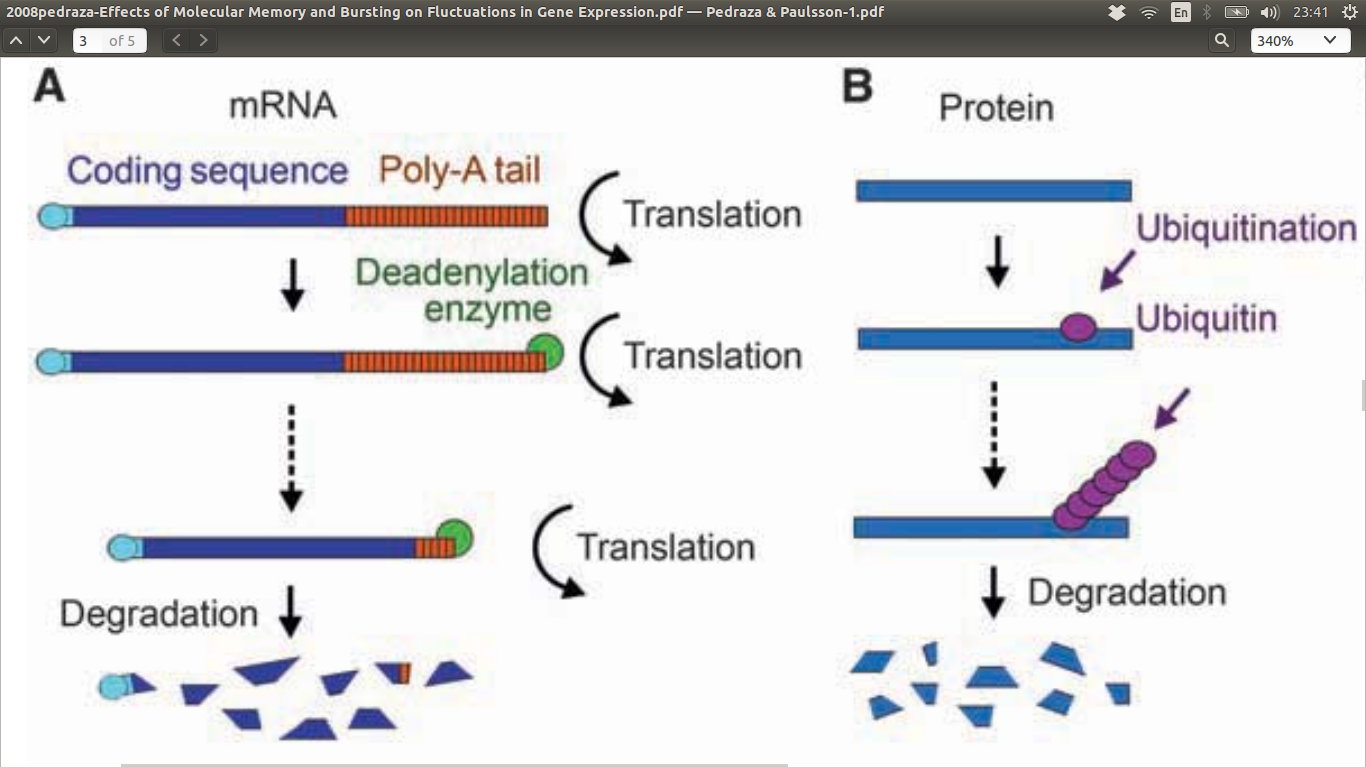
\includegraphics[width=16cm]{bur-examples}
  \caption[Examples of bursting and senescence in gene expression]{\label{fig:bur-examples} Examples of bursting and senescene in gene expression. (Left) Promoter where many transcription factors bind in successive steps taking a random time $T$. When the complex is bound to the promoter, a random number $b$ of transcription events occur in a time much shorter than $T$. (Right) Senescene in eukaryotic mRNA occurs when their poly(A) tail (an additional stretch of mRNA that is not part of the protein coding sequence) is sequentially removed before the coding sequence is degraded. Translation can occur while the poly(A) tail is removed. From \cite{pedraza08}.}
\end{figure}

\section{mRNA bursts}
Let the mRNA be produced in bursts of random size $b$, the degradation and protein creation occur one at a time with exponential waiting times (single-step Poisson processes). In this case the only modification with respect to the ``standard model'' [eq. \eqref{eq:mas-simple_det_1}] is the $D_{11}$ term in the matrix $\mathbf{D}$ of the FDT, which by definition is

\begin{equation}
  \label{eq:mrnab1}
  D_{11}=\frac{1}{\langle n_1\rangle^2}\sum_k(s_1^k)^2r_k(\mathbf{n}).
\end{equation}

All the possible $k$ reactions include all the creation bursts and the reaction of degradation whose rate is $\langle n_1 \rangle/\tau_1$ and has a value of $s_1=-1$, then

\begin{equation}
  \label{eq:mrnab2}
  \sum_k(s_1^k)^2r_k = \frac{\langle n_1 \rangle}{\tau_1} + \sum_{k}(s_1^{k})^2r_{k},
\end{equation}

where now the index $k$ runs over all the synthesis reactions only. We can rewrite the second term as

\begin{equation*}
  \sum_k(s_1^k)^2r_k=\sum_kr_k\sum_k\left(\frac{r_k}{\sum_kr_k}\right)(s_1^k)^2,
\end{equation*}

where the sum over the term in parentheses results in $1$. This term can be interpreted as the probability that the upcoming reaction turns out to be the $k^{\text{th}}$ one. Writing it as $\rho_k$

\begin{equation*}
  \sum_k(s_1^k)^2r_k=\sum_kr_k\sum_k\rho_k(s_1^k)^2,
\end{equation*}

but $s_1^k$ is the burst size for the $k^{\text{th}}$ synthesis reaction. Therefore the inner sum of the previous equation is actually an average over all the possible burst sizes, hence

\begin{equation}
  \label{eq:mrnab4}
  \sum_k(s_1^k)^2r_k=\sum_kr_k\langle b^2 \rangle=\left(\langle b\rangle^2+\sigma_b^2\right)\sum_kr_k,
\end{equation}

and using a similar trick we get

\begin{equation*}
  \begin{split}
    \sum_kr_k&=\sum_kr_ks_1^k\frac{\sum_kr_k}{\sum_kr_ks_1^k}=\sum_kr_ks_1^k\left(\sum_k\left(\frac{r_k}{\sum_kr_k}\right)s_1^k\right)^{-1}\\
    &=\sum_kr_ks_1^k\left(\sum_k\rho_ks_1^k\right)^{-1}=\frac{1}{\langle b\rangle}\sum_kr_ks_1^k.
  \end{split}
\end{equation*}

If the system is in steady state, the net synthesis rate equal the degradation rate. Therefore

\begin{equation*}
  \sum_kr_ks_1^k = \frac{\langle n_1\rangle}{\tau_1},
\end{equation*}

obtaining

\begin{equation*}
   \sum_kr_k = \frac{\langle n_1\rangle}{\langle b\rangle\tau_1}.
\end{equation*}

Replacing this on eq. \eqref{eq:mrnab4}, then on eq. \eqref{eq:mrnab2}, and finally on \eqref{eq:mrnab1} we get

\begin{equation}
  \label{eq:d11}
  D_{11}=\frac{1}{\langle n_1\rangle^2}\left(\frac{\langle n_1\rangle}{\tau_1}+\frac{\langle n_1\rangle}{\langle b\rangle\tau_1}\left(\langle b\rangle^2+\sigma_b^2\right)\right) = \frac{1}{\tau_1\langle n_1\rangle}\left( 1+ \langle b\rangle\left(1+\frac{\sigma_b^2}{\langle b\rangle^2}\right)\right)
\end{equation}

Hence, the matrices for the FDT are

\begin{equation*}
  \mathbf{D} = 
  \begin{pmatrix}
    D_{11} & 0 \\
    0 & \frac{2}{\tau_2\langle n_2\rangle}
  \end{pmatrix}, \quad
  \mathbf{M} =
  \begin{pmatrix}
    \frac{1}{\tau_1} & 0 \\
    -\frac{1}{\tau_2} & \frac{1}{\tau_2}
  \end{pmatrix},
\end{equation*}

where $D_{11}$ is given by eq. \eqref{eq:d11}. By solving the linear system $\mathbf{M}\mathbf{\eta} + \mathbf{\eta M}^T+\mathbf{D}=0$ we obtain the following expression for the noise in protein number

\begin{equation*}
  \eta_{22}=\frac{1}{\langle n_2\rangle} + \frac{1}{\langle n_1\rangle} \frac{\tau_1}{\tau_1 + \tau_2} \frac{\langle b\rangle\left(1+\nicefrac{\sigma_b^2}{\langle b\rangle^2}\right)+1}{2}.
\end{equation*}

Recall that this holds under the assumption that the times between creation events are exponentially distributed. The noise in the number of proteins does not depend on the details of the distribution of $b$, but only on its noise. In the noise propagated from mRNA, apart from the time averaging factor, there is a \textit{coarse graining} factor that captures how fluctuations are generated. In the following sections we will derive the noise in the number of proteins for arbitrary waiting times.

\section{Arbitrary distribution of creation times}

Suppose a creation event occurred at $t=0$, and let $f(t)$ be the PDF of a creation event happening at time $t$ after the last event, i.e. $P(t\in[T,T+dt])=f(T)dt$. Hence

\begin{equation*}
P(n=0|t=T) = P(t>T) = 1 - P(t<T) = 1 - F(T),
\end{equation*}

where $n$ is number of creation events and $F$ is the CDF associated to $f$. Also, for a creation event to have happened before time $t=T$, there must be a creation at a time $t_1$ such that $0<t_1<T$ and none during the remaining ($T-t_1$) time. This leads to the following equation

\begin{equation*}
  \begin{split}
    P(n=1|t=T) &= \int_0^TP(t=t_1)P(t>T-t_1)\mathrm{d}t_1 \\
    &= \int_0^Tf(t_1)(1-F(T-t_1))\mathrm{d}t_1=f\ast (1-F)|_T.
  \end{split}
\end{equation*}

The asterisk denotes the convolution product. Following a similar argument, we obtain for an arbitrary number of events

\begin{equation}
  \label{eq:nconvs}
  \begin{split}
    P(n=N|t=T) &= f\ast P(n=N-1|t)|_T = f\ast f\ast P(n=N-2|t)|_T \\
    &= \cdots = \underbrace{f\ast\cdots\ast f}_{n \text{ times}}\ast P(n=0,t)|_T = \underbrace{f\ast\cdots\ast f}_{n \text{ times}}\ast (1-F)|_T.
  \end{split}
\end{equation}

Since the convolutions are difficult to deal with, we will use the Laplace transform and solve on the Laplace space. The property that $\mathcal{L}(f\ast g) = \hat{f}\cdot\hat{g}$, where $\hat{f}\coloneqq\mathcal{L}(f)$ will make the problem much simpler.

Aplying $\mathcal{L}$ to eq. \eqref{eq:nconvs} we get

\begin{equation*}
  \hat{P}(n,s) = \hat{f}^n(s)\mathcal{L}(1-F)(s).
\end{equation*}

It can be easily shown that $\hat{F} = \hat{f}/s$ and $\hat{1} = 1/s$, applying these properties,

\begin{equation}
  \label{eq:lapP}
  \hat{P}(n,s) = \frac{1}{s}\hat{f}^n(s)(1-\hat{f}(s)).
\end{equation}

To find the moments and the noise, we will use the moment generating function, as defined on \eqref{def:mom_gen}. It will be denoted as $G(z,s)$.

\begin{equation}
  \label{eq:lapG}
  \hat{G}(z,s) \coloneqq \sum_{n=0}^{\infty}z^n\hat{P}(n,s) = \frac{1}{s}(1-\hat{f}(s))\sum_{n=0}^{\infty}(z\hat{f})^n=\frac{1-\hat{f}(s)}{s(1-z\hat{f}(s))}.
\end{equation}

The geometric series convereges in this case because $\hat{f}(s)\leq1$ and we will evaluate $z$ at $1$. The first and second derivatives of $G$ in Laplace space are given by

\begin{equation}
  \label{eq:lapavn}
  \langle\hat{n}\rangle(s) = \left.\frac{\partial\hat{G}(z,s)}{\partial z}\right|_1 = \frac{\hat{f}(s)}{s(1-\hat{f}(s))}.
\end{equation}

\begin{equation}
  \label{eq:lapvarn}
  \langle\hat{n}(\hat{n}-1)\rangle(s) = \left.\frac{\partial^2\hat{G}(z,s)}{\partial z^2}\right|_1 = \frac{2}{s}\left(\frac{\hat{f}(s)}{1-\hat{f}(s)}\right)^2.
\end{equation}

It could also be proven that

\begin{equation}
  \label{eq:lapfprop}
  \hat{f}(0) = 1, \quad \left.\frac{\mathrm{d}\hat{f}(s)}{\mathrm{d}s}\right|_0=-\langle t\rangle,\quad \left.\frac{\mathrm{d}^2\hat{f}(s)}{\mathrm{d}s^2}\right|_0=\langle t^2\rangle.
\end{equation}

Therefore, we can obtain the moments by applying the inverse Laplace transform to eqs. \eqref{eq:lapavn}-\eqref{eq:lapvarn}, and using properties \eqref{eq:lapfprop}. For the expected value

\begin{equation}
  \langle n\rangle(t) = \mathcal{L}^{-1}(\langle\hat{n}\rangle(s))=\frac{1}{2i\pi}\oint e^{st}\frac{\hat{f}(s)}{s(1-\hat{f}(s))}\mathrm{d}s
\end{equation}

The integral can be solved by residues. Since $\hat{f}(0)=1$, there is a pole of order $2$ in $s=0$. To find the residues of a pole $c$ of order $m$ of the function $f$, the residue is given by

\begin{equation}
  \label{eq:residues}
  \text{Res}_c(f)=\frac{1}{(m-1)!}\lim_{z\to c}\frac{\mathrm{d}^{m-1}}{\mathrm{d}z^{m-1}}((z-c)^mf(z)).
\end{equation}

Then

\begin{equation*}
  \begin{split}
    \langle n\rangle(t)&=\text{Res}_0\frac{e^{st}}{s}\frac{\hat{f}(s)}{1-\hat{f}(s)}=\lim_{s\to0}\frac{\mathrm{d}}{\mathrm{d}s}\frac{se^{st}\hat{f}(s)}{1-\hat{f}(s)}\\
    & = \lim_{s\to0}\frac{e^{st}}{(\hat{f}(s)-1)^2}\left[(1+st)(\hat{f}(s)-1)\hat{f}(s) + s\hat{f}'(s)\right].
  \end{split}
\end{equation*}

To find the limit we have to apply L'Hospital rule twice. After some algebra the obtained result is

\begin{equation}
  \label{eq:aven}
  \langle n\rangle(t)=\frac{\hat{f}''(0)}{2(\hat{f}'(0))^2}-\frac{t}{\hat{f}'(0)}-1=\frac{t}{\langle t\rangle}+\left(\frac{\langle t^2\rangle}{2\langle t\rangle^2}-1\right).
\end{equation}

For the second moment, inverting eq. \eqref{eq:lapvarn} we obtain

\begin{equation*}
  \begin{split}
    \langle n(n-1)\rangle(t)&=\frac{1}{2i\pi}\oint e^{st}\frac{2}{s}\left(\frac{\hat{f}(s)}{1-\hat{f}(s)}\right)^2\mathrm{d}s=\text{Res}_0\frac{2}{s}\left(\frac{\hat{f}(s)}{1-\hat{f}(s)}\right)^2\\
&=\lim_{s\to0}\frac{\mathrm{d}^2}{\mathrm{d}s^2}e^{st}\left(\frac{s\hat{f}(s)}{1-\hat{f}(s)}\right)^2,
  \end{split}
\end{equation*}

where we used eq. \eqref{eq:residues} to find the residue of a pole of order $3$. After doing the necessary algebra and applying the L'Hospital rule three times we get

\begin{equation*}
  \langle n(n-1)\rangle(t)=\frac{t^2}{\langle t\rangle^2}+\frac{4t}{\langle t\rangle}\left(\frac{\langle t^2\rangle}{2\langle t\rangle^2}-1\right)+2\left(1-\frac{\langle t^2\rangle}{\langle t\rangle^2}+\frac{3\langle t^2\rangle^2}{4\langle t\rangle^4}+\frac{\langle t^3\rangle}{3\langle t\rangle^3}\right).
\end{equation*}

Combining with eq. \eqref{eq:aven} we obtain the variance

\begin{equation}
  \label{eq:stdn}
  \sigma_n^2(t) = \frac{t}{\langle t\rangle}\left(\frac{\langle t^2\rangle}{\langle t\rangle^2}-1\right)+\left(-\frac{\langle t^2\rangle}{2\langle t\rangle^2} + \frac{5\langle t^2\rangle^2}{4\langle t\rangle^4}-\frac{2\langle t^3\rangle}{3\langle t\rangle^3}\right).
\end{equation}

The second terms of eqs. \eqref{eq:aven} and \eqref{eq:stdn} represent the fact that, in general, the distribution for the events depend on the initial time. They are exactly zero if times were exponentially distributed, consistent with the memorylessness property\footnote{This can be easily proven using the following property: if $X$ is an exponential random variable, then $\langle X^m\rangle = n!/\lambda^m$, for $m\in\mathbb{Z}^+$.}. If we assume that the starting time is far in the past these terms are negligible. This yields

\begin{equation*}
  \langle n\rangle = \frac{t}{\langle t\rangle},\quad\quad\sigma_n^2 = \frac{t}{\langle t\rangle}\left(\frac{\langle t^2\rangle}{\langle t\rangle^2}-1\right).
\end{equation*}

Using both equations,

\begin{equation*}
  \sigma_n^2 = \frac{t}{\langle t\rangle}\left(\frac{\langle t^2\rangle - \langle t\rangle^2}{\langle t\rangle^2}\right) = \frac{t}{\langle t\rangle}\eta_t^2 = \langle n\rangle\eta_t^2.
\end{equation*}

Hence

\begin{equation}
  \label{eq:noisen1}
  \eta_n^2=\frac{1}{\langle n\rangle}\eta_t^2, \quad \text{with}\quad \langle n\rangle = \frac{t}{\langle t\rangle}.
\end{equation}

Now we will include the effect of bursts of creation. Let $n$ be the number of creation events (meaning the number of bursts, not the total number of molecules created), and let $b_i$ be burst size for the $i^{\text{th}}$ events. Both $n$ and $b_i$ are random variables, and all the $b_i$s follows the same probability distribution. Then, the number of molecules created is

\begin{equation}
  \label{eq:xtotal}
  x\coloneqq\sum_{i=0}^nb_i.
\end{equation}

It is a sum of a random number of random variables. Denoting the probability mass function of $x$ as $P_x(x)$, and using the definition of the characteristic function $\phi(s)$ [see sec. \ref{sec:con-charac_func}] we get

\begin{equation*}
  \phi(s) \coloneqq \langle e^{xs}\rangle_x = \sum_{a=0}^\infty e^{xs}P_x(x=a).
\end{equation*}

Using the total probability theorem, we can write it as

\begin{equation}
  \label{eq:charac1}
  \begin{split}
    \phi(s) &= \sum_{a=0}^\infty e^{xs}\sum_{n=0}^\infty P_x(x=a|n)P(n) = \sum_{n=0}^\infty\left(\sum_{a=0}^\infty e^{xs}P_x(x=a|n)\right)P(n)\\ 
&= \sum_{n=0}^\infty \langle e^{xs}\rangle_{x|n} P(n).
  \end{split}
\end{equation}

$\langle\quad\rangle_x$ denotes average with respect to the distribution of $x$. Using eq. \eqref{eq:xtotal} we obtain

\begin{equation*}
  \langle e^{xs}\rangle_{x|n} = \left\langle e^{s\sum_{i=0}^nb_i} \right\rangle_b = \left\langle \prod_{i=0}^ne^{sb_i}\right\rangle_b.
\end{equation*}

Assuming independence between the different burst sizes $b_i$ and using eq. \eqref{eq:con-mom_ind} we get

\begin{equation*}
  \langle e^{xs}\rangle_{x|n} =  \prod_{i=0}^n\langle e^{sb_i}\rangle_b,
\end{equation*}

and since all the $b_i$s follow the same distribution, the product is independent of $i$

\begin{equation*}
  \langle e^{xs}\rangle_{x|n} = \prod_{i=0}^n\langle e^{sb}\rangle_b = \langle e^{sb}\rangle_b^n.
\end{equation*}.

Replacing this result in eq. \eqref{eq:charac1},

\begin{equation*}
  \phi(s) = \sum_{n=0}^\infty \langle e^{sb}\rangle_b^n P(n) = \left\langle\langle e^{sb}\rangle_b^n\right\rangle_n,
\end{equation*}

where $\langle\quad\rangle_n$ denotes average with respect to the distribution of events. Now we find the moments using the properties of the characteristic function

\begin{equation}
  \label{eq:avex}
  \langle x\rangle = \left.\frac{\mathrm{d}\phi(s)}{\mathrm{d}s}\right|_0 = \left.\frac{\mathrm{d}}{\mathrm{d}s}\left\langle\langle e^{bs}\rangle_b^n\right\rangle_n\right|_0 = \left.\left\langle n\langle e^{bs}\rangle_b^{n-1}\langle b e^{bs}\rangle_b\right\rangle_n\right|_0 = \left\langle n\langle b\rangle_b\right\rangle_n = \langle n\rangle_n\langle b\rangle_b,
\end{equation}

The average number of molecules produced is thus the mean number of bursts times the mean burst size. For the second moment,

\begin{equation*}
  \begin{split}
    \langle x^2\rangle &= \left.\frac{\mathrm{d^2}\phi(s)}{\mathrm{d}s^2}\right|_0 = \left.\frac{\mathrm{d}\phi(s)}{\mathrm{d}s}\left\langle n\langle e^{bs}\rangle_b^{n-1}\langle b e^{bs}\rangle_b\right\rangle_n\right|_0\\
  &= \left.\left\langle n(n-1)\langle e^{bs}\rangle^{n-2}_b\langle be^{bs}\rangle^2_b+n\langle e^{bs}\rangle^{n-1}_b\langle b^2e^{bs}\rangle_b\right\rangle_n\right|_0\\
  &=\langle n^2\rangle_n\langle b\rangle_b^2-\langle n\rangle_n\langle b\rangle_b^2+\langle n\rangle_n\langle b^2\rangle_b.
  \end{split}
\end{equation*}

Using the previous result with eq. \eqref{eq:avex} to find the variance, we get

\begin{equation*}
  \begin{split}
    \sigma_x^2 &= \langle n^2\rangle_n\langle b\rangle_b^2-\langle n\rangle_n\langle b\rangle_b^2+\langle n\rangle_n\langle b^2\rangle_b - \langle n\rangle_n^2\langle b\rangle_b^2\\
    &=\langle b\rangle_b^2\left(\langle n^2\rangle_n-\langle n\rangle^2_n\right) + \langle n\rangle_n\left(\langle b^2\rangle_b-\langle b\rangle_b^2\right)\\
    &=\langle b\rangle_b^2\sigma_n^2 + \langle n\rangle_n\sigma_b^2.
  \end{split}
\end{equation*}

Dividing by $\langle x\rangle^2=\langle n\rangle_n^2\langle b\rangle_b^2$,

\begin{equation*}
  \eta_x^2=\frac{\sigma_n^2}{\langle n\rangle_n^2} + \frac{\sigma_b^2}{\langle n\rangle_n\langle b\rangle_b^2} = \eta_n^2+\frac{1}{\langle n\rangle_n}\eta_b^2.
\end{equation*}

Replacing eq. \ref{eq:noisen1} we obtain

\begin{equation}
  \label{eq:noisex}
  \eta_x^2=\frac{1}{\langle n\rangle}\left(\eta_t^2+\eta_n^2\right)=\frac{\langle b\rangle\left(\eta_t^2+\eta_n^2\right)}{\langle x\rangle},
\end{equation}

where

\begin{equation}
  \langle x\rangle = \langle b\rangle\frac{t}{\langle t\rangle}.
\end{equation}

This result holds for a pure birth process.

\section{Decay of molecules}

We include the decay of molecules considering their partitioning during cell division. Let $P_\text{Dr}(l|m)$ be the probability of finding $l$ molecules in volume fraction $r$ given that there are $m$ molecules before division.

Assuming that each molecule segregates independently, and that the probability of arriving at a volume is proportional to it we obtain a binomial distribution

\begin{equation*}
  P_\text{Dr}(l|m) = {m\choose l}r^l(1-r)^{m-l}.
\end{equation*}

For a fixed volume fraction $r$, let $P_\text{Br}(m)$ and $P_\text{Ar}(m)$ be the probabilities of having $m$ molecules before and after division, respectively. Then

\begin{equation*}
  P_\text{Ar}(l) = \sum_{m=0}^\infty P_\text{Dr}(l|m)P_\text{Br}(m) = \sum_{m=0}^\infty {m\choose l}r^l(1-r)^{m-l}P_\text{Br}(m).
\end{equation*}

Multiplying by $z^l$ and summing we get the moment generating function $G_\text{Ar}(z)$

\begin{equation}
  \label{eq:binomG}
  \begin{split}
    G_\text{Ar}(z) &= \sum_{l=0}^\infty z^l\sum_{m=0}^\infty {m\choose l}r^l(1-r)^{m-l}P_\text{Br}(m)\\
    &= \sum_{m=0}^\infty\left(\sum_{l=0}^\infty (zr)^l(1-r)^{m-l}\right)P_\text{Br}(m).\\
    &= \sum_{m=0}^\infty(zr+1-r)^{m}P_\text{Br}(m),
  \end{split}
\end{equation}

The number of molecules of at the end of a growth stage (with distribution $P_\text{Br}$) equals the number of molecules at the beginning (with distribution $P_\text{Ar}$) plus the number of molecules created during the cycle (with distribution $P_{x,\tau} \coloneqq P_x|_{t=\tau}$). Assuming that both random variables as independent, and recalling that the PMF of the sum of random variables is the convolution of the individual PMFs,

\begin{equation*}
  P_\text{Br}(m) = P_\text{Ar}\ast P_{x,\tau}(m).
\end{equation*}

Thus,

\begin{equation*}
  G_\text{Br}(z) = G_\text{Ar}(z)G_{x,\tau}(z).
\end{equation*}

From the properties of $G$ and the previous equation the moments can be obtained. The mean is given by

\begin{equation}
  \label{eq:bur-aveBr}
  \langle n\rangle_\text{Br} = \left.\frac{\partial G_\text{Br}(z)}{\partial z}\right|_1 = G_\text{Ar}(1)\left.\frac{\partial G_{x,\tau}(z)}{\partial z}\right|_1 + \left.\frac{\partial G_\text{Ar}(z)}{\partial z}\right|_1G_{x,\tau}(1) = \langle m\rangle_{x,\tau} + \langle m\rangle_\text{Ar},
\end{equation}

and from eq. \eqref{eq:binomG},

\begin{equation*}
  \begin{split}
  \left.\frac{\partial G_\text{Ar}(z)}{\partial z}\right|_1 &= \langle m\rangle_\text{Ar} = \left.\frac{\partial}{\partial z} \sum_{m=0}^\infty(zr+1-r)^mP_\text{Br}(m)\right|_1\\
&= \left.\sum_{m=0}^\infty m(zr+1-1)^{m-1}rP_\text{Br}(m)\right|_1\\
&= r\sum_{m=0}^\infty mP_\text{Br}(m) = r\langle m\rangle_\text{Br}.
  \end{split}
\end{equation*}
  
Therefore

\begin{equation}
  \label{eq:aveBrAr}
  \langle m\rangle_\text{Br} = \frac{1}{1-r}\langle m\rangle_{x,\tau},\quad\quad \langle m\rangle_\text{Ar} = r\langle n\rangle_\text{Br} = \frac{r}{1-r}\langle m\rangle_{x,\tau}.
\end{equation}

Now we find the variance. Differentiating twice we obtain

\begin{equation}
  \label{eq:2Br}
  \begin{split}
    \langle m(m-1)\rangle_\text{Br} &= \left.\frac{\partial^2 G_\text{Br}(z)}{\partial z^2}\right|_1\\
    &=G_\text{Ar}(1)\left.\frac{\partial^2 G_{x,\tau}(z)}{\partial z^2}\right|_1 + \left.\frac{\partial^2 G_\text{Ar}(z)}{\partial z^2}\right|_1G_{x,\tau}(1) + 2\left.\frac{\partial G_\text{Ar}(z)}{\partial z}\right|_1\left.\frac{\partial G_{x,\tau}(z)}{\partial z^2}\right|_1\\
    &=\langle m(m-1)\rangle_{x,\tau}+\langle m(m-1)\rangle_\text{Ar}+2\langle m\rangle_{x,\tau}\langle m\rangle_\text{Ar},
  \end{split}
\end{equation}

and from eq. \eqref{eq:binomG}

\begin{equation}
  \label{eq:2Ar}
  \begin{split}
    \langle m(m-1)\rangle_\text{Ar} &= \left.\frac{\partial^2}{\partial z^2}\sum_{m=0}^\infty(zr+1-r)^mP_\text{Br}(n)\right|_1\\
    &= \left.\sum_{m=0}^\infty m(m-1)(zr+1-r)^{m-2}r^2P_\text{Br}(n)\right|_1 = r^2\langle n(n-1)\rangle_\text{Br}.
  \end{split}
\end{equation}

For any random variable $x$, we can write $\langle x(x-1)\rangle = \sigma_x^2 - \langle x\rangle + \langle x\rangle^2$. Using this on eqs. \eqref{eq:2Br} and \eqref{eq:2Ar} we get

\begin{equation*}
  \begin{split}
  \sigma^2_\text{Br}- \langle m\rangle_\text{Br} + \langle m\rangle^2_\text{Br} &= \left( \sigma^2_{x,\tau} - \langle m\rangle_{x,\tau} + \langle m\rangle_{x,\tau}^2\right)\\
&+ 2\left(r\langle m\rangle_\text{Br}\right)\left[(1-r)\langle m\rangle_\text{Br}\right]+r^2\left(\sigma^2_\text{Br}- \langle m\rangle_\text{Br} + \langle m\rangle^2_\text{Br}\right).
  \end{split}
\end{equation*}

After some algebra the expression can be reduced to

\begin{equation}
  \label{eq:sigmaBr}
  \sigma^2_\text{Br} = \frac{1}{1-r^2}\sigma^2_{x,\tau}+\frac{r}{1+r}\langle m\rangle_\text{Br}
\end{equation}

Dividing by $\langle m\rangle_\text{Br}^2$ and using eq. \ref{eq:aveBrAr} we get

\begin{equation}
  \label{eq:bur-etaBr}
  \begin{split}
    \eta_\text{Br}^2 &= \frac{1}{1-r^2}\sigma_{x,\tau}^2\frac{(1-r)^2}{\langle m\rangle_{x,\tau}^2} + \frac{r}{1+r}\langle m\rangle_\text{Br}\\
    & = \frac{1-r}{1+r}\eta_{x,\tau}^2+\frac{r}{1+r}\frac{1}{\langle n\rangle_\text{Br}}
  \end{split}
\end{equation}

Also, from eqs. \ref{eq:2Ar} and \ref{eq:sigmaBr} we get

\begin{equation}
  \begin{split}
    \sigma^2_\text{Ar} - \langle m\rangle_\text{Ar} + \langle m\rangle_\text{Ar}^2 &= r^2\left(\sigma^2_\text{Br}- \langle m\rangle_\text{Br} + \langle m\rangle^2_\text{Br}\right)\\
  &=r^2\left(\frac{1}{1-r^2}\sigma^2_{x,\tau}+\frac{r}{1+r}\langle m\rangle_\text{Br}\right)-r^2\langle m\rangle_\text{Br} + r^2\langle m\rangle^2_\text{Br}
  \end{split}
\end{equation}

Using eq. \ref{eq:aveBrAr} and after a little algebra we get

\begin{equation}
  \sigma^2_\text{Ar} = \frac{r^2}{1-r^2}\sigma^2_{x,\tau}+\frac{1}{1+r}\langle m\rangle_\text{Ar},
\end{equation}

hence, dividing by $\langle m\rangle_\text{Ar}^2$ and using eq. \eqref{eq:aveBrAr},

\begin{equation}
  \begin{split}
    \eta^2_\text{Ar} &= \frac{r^2}{1-r^2}\sigma^2_{x,\tau}\left(\frac{1-r}{r\langle m\rangle_{x,\tau}}\right)^2+\frac{1}{1+r}\frac{1}{\langle m\rangle_\text{Ar}}\\
    &=\frac{1-r}{1+r}\eta^2_{x,\tau}+\frac{1}{1+r}\frac{1}{\langle m\rangle_\text{Ar}}.
  \end{split}
\end{equation}

From eqs. \eqref{eq:bur-aveBr} and \eqref{eq:aveBrAr}, we have $\langle n\rangle_{x,\tau}=\langle n\rangle_{Br}(1-r)$. Replacing on eq. \eqref{eq:noisex}

\begin{equation*}
  \eta^2_{x,\tau} = \frac{\langle b\rangle(\eta^2_t+\eta^2_b)}{(1-r)\langle n\rangle_{Br}},
\end{equation*}

and replacing this on eq. \eqref{eq:bur-etaBr} we obtain

\begin{equation*}
  \eta^2_{Br} = \frac{\langle b\rangle(\eta^2_t+\eta^2_b) + r}{(1+r)\langle n\rangle_{Br}}.
\end{equation*}

The continuous decay of molecules can be approximated by considering division in the limit where $r\to 1$, that is, when the lost volume fraction is very small. In this case,

\begin{equation*}
  \eta^2 = \lim_{r\to 1}\eta^2_{Br} = \frac{\langle b\rangle(\eta^2_t+\eta^2_b) + 1}{2\langle n\rangle}.
\end{equation*}

In the model of transcription and translation this corresponds to the noise in mRNA number. The noise in protein number can be found immediately keeping in mind that, as we saw on chapter \ref{ch:fdt}, the noise in the number of protein is composed of its intrinsic Poissonian component ($1/\langle p\rangle$), and the transmitted noise from mRNA modulated by the time averaging factor, i.e.

\begin{equation*}
  \eta^2_p = \frac{1}{\langle p\rangle} + \frac{\langle b\rangle(\eta^2_t+\eta^2_b) + 1}{2}\frac{1}{\langle m\rangle}\frac{\tau_m}{\tau_m+\tau_p}.
\end{equation*}

Therefore, by considering the bursting and general random timing between creation events in the number of mRNAs, an additional factor arises. The authors of \cite{pedraza08} have called it coarse graining factor because it is overlooked with the usual approximations. According to the previous eq., noise can be reduced by having narrowly distributed gestation period (e.g. by introducing more steps). Also, there are many ways in which the same noise is obtained, e.g. with a narrow distribution of times and a wide one of bursts, or viceversa. Hence, the models that overlook these variables and have estimated quantities based on some prior assumptions may be wrong. For example, the noise that has been attributted to a high number of mRNAs, or to the effect of time averaging could have been caused by a narrowly distributed time between events.

\section{Senescence of mRNA}

Suppose that mRNAs are created at a constant rate $\lambda_1$ and that they senesce through a sequence of $N$ steps labeled as $X_1,X_2,\dotsc,X_N$. Thus, the states and their transitions are

\begin{equation*}
  \text{Transcription} \rightarrow X_1 \rightarrow X_2 \rightarrow \dots \rightarrow X_N \rightarrow \text{Degradation}
\end{equation*}

The number of mRNA molecules in each step is labeled as $x_i$ for $1\leq i\leq N$. Let the rate of transcription be $\lambda_1$ and assume that the rates of transition $\beta_1$ per mRNA between the states are the same. The possible transtions in the state space are thus

\begin{equation}
  \begin{split}
    x_1&\xrightarrow{\lambda_1}x_1+1,\\
    \{x_i,x_{i+1}\}&\xrightarrow{\beta_1x_i} \{x_i-1,x_{i+1}+1\},\quad \text{for}\quad1\leq i\leq N-1,\\
    x_N&\xrightarrow{\beta_1x_N} x_N-1.
  \end{split}
\end{equation}

The first line denotes transcription, the second denotes transitions between states and the third refers to degradation. Now, let $x_{N+1}$ be the number of proteins in the cell and suppose that independently of the current state of the mRNA molecules, they are translated with the same rate $\lambda_2$ per mRNA. The possible transitions for the proteins are

\begin{equation*}
  \begin{split}
    x_{N+1} &\xrightarrow{\lambda_2\sum_{i=1}^Nx_i} x_{N+1}+1,\\
    x_{N+1} &\xrightarrow{\beta_2x_{N+1}}x_{N+1}-1,
  \end{split}
\end{equation*}

where $\beta_2$ is their degradation rate. Then, the average dynamics are

\begin{equation*}
  \begin{split}
    \dot{\langle x_1\rangle} &= \lambda_1 -\beta_1\langle x_1\rangle,\\
    \dot{\langle x_{i+1}\rangle} &= \beta_1\left(\langle x_i\rangle - \langle x_{i+1}\rangle\right)\quad\text{for}\quad 1\leq i\leq N,\\
    \dot{\langle x_{N+1}\rangle} &= \lambda_2\sum_{i=1}^N\langle x_i\rangle-\beta_2\langle x_{N+1}\rangle.
  \end{split}
\end{equation*}

At steady state we get

\begin{equation*}
  \begin{split}
    \langle x_1\rangle &= \frac{\lambda_1}{\beta_1},\\
    \langle x_{i+1}\rangle &= \langle x_i\rangle\quad\text{for}\quad 1\leq i\leq N-1,\\
    \langle x_{N+1}\rangle &= \frac{\lambda_2}{\beta_2}\sum_{i=1}^N\langle x_i\rangle.
  \end{split}
\end{equation*}

Hence

\begin{equation*}
  \langle x_i\rangle = \lambda_1\tau_1\quad\text{for}\quad 1\leq i\leq N,
\end{equation*}

where $\tau_1 \coloneqq 1/\beta_1$. Denoting the total mRNA as $m=\sum_{i=1}^Nx_i$ and taking the average,

\begin{equation*}
  \langle m\rangle = \sum_{i=1}^N\langle x_i\rangle = \lambda_1\tau_1n = \lambda_1\tau_m
\end{equation*}

where $\tau_m\coloneqq n\tau_1$. With the previous results the coefficients of the matrices $\mathbf{M}$ and $\mathbf{D}$ of the FDT can be found, replaced in the equation and solved for the noises. Following this procedure, we obtain the following expression for the noise in the number of proteins

\begin{equation*}
  \eta_p^2= \frac{1}{\langle p\rangle}+\frac{1}{\langle m\rangle} \left[1+\frac{\tau_p}{\tau_m}\left(\left(\frac{\tau_pN}{\tau_m+\tau_pN}\right)^N-1\right)\right].
\end{equation*}

The noise for the total mRNA can be found using the properties of time averaging. If we let $\tau_p\ll\tau_m$ the proteins respond immediately to changes in mRNA. Consequently, the transmitted fluctuations from the mRNA are completely reproduced by them and we get

\begin{equation*}
  \eta_m^2 = \frac{1}{\langle m\rangle}.
\end{equation*}

This is a very surprising result, by letting the mRNA senesce through multiple steps before being degraded, $\eta_m$ remains Poissonian but the time averaging factor in $\eta_p$ is modified. The noise is reduced with a larger number of senescence steps $N$ and viceversa, as can be proved taking the limits as $N\to 0$ and $N\to \infty$, or plotting as a function of $N$. If proteins senesce, the noise would instead be increased with a larger number of steps.

This nonintuitive result reasserts the conclusion of the previous section. There are many mechanisms that affect the noise. For that reason, it is not correct to fit the parameters and the variables of some models under assumptions that may not hold with a high probability. Altough with this method the models predict the experimental results, the origin of the noise is attributed to factors that may not be the actual ones. For instance, noise that arises from senescence can be attributed only to the low numbers of mRNAs.


\chapter{Effects of cell division}
\label{ch:div}

When the cell divides, all the components (organelles, proteins, genetic material, etc.) must be distributed among the daughter cells. Nevertheless, the assymetries on partition are an important source of noise even for components present at high numbers. In this chapter we will explore some general mechanisms of partition of molecules during cell division and how they can affect noise statistics.

This chapter follows the work done by D. Huh and J. Paulsson in \cite{huh11b}.

\section{Characterizing the noise arising from cell division}

Let $x = l+r$ be the number of copies of some component (e.g. a certain protein) for a dividing cell, with $l$ and $r$ being the number of copies each daughter cell recieves. Also, let $v$ be the number of molecules of some component that affects the partition such as vacuoles or splindles. On average, we expect the molecules to distribute symmetrically. Therefore

\todo[inline]{Explain vacuoles and spindles here?}

\begin{equation}
  \label{eq:div-even}
  \langle l\rangle = \langle r\rangle = \frac{\langle x\rangle}{2}.
\end{equation}

We will find the noise for $l$\footnote{It does not matter if we choose $r$ or $l$ since there is not preference for one of the daughter cells}. Using the law of total variance (eq. \eqref{eq:con-total_var}), the variance of $l$ is given by

\begin{equation*}
  \sigma^2(l) = \sigma^2\left(\langle l|x,v\rangle\right) + \left\langle\sigma^2(l|x,v)\right\rangle.
\end{equation*}

From eq. \eqref{eq:div-even}, $\langle l|x,v\rangle = \nicefrac{x}{2}$, using this and dividing by $\langle l\rangle^2 = \nicefrac{\langle x\rangle^2}{4}$ we get

\begin{equation}
  \label{eq:div-noises}
  \begin{split}
    \eta^2(l) &= 4\frac{\sigma^2\left(\nicefrac{x}{2}\right)}{\langle x\rangle^2}+\frac{\langle\sigma^2(L|x,v)\rangle}{\langle L\rangle^2}\\
    &=\eta^2(x) + Q_x^2,
  \end{split}
\end{equation}

where we used eq. \eqref{eq:con-var_const}. The term $Q_x$, defined as

\begin{equation}
  \label{eq:div-Q}
  Q_x^2 \coloneqq \frac{\langle\sigma^2(L|x,v)\rangle}{\langle L\rangle^2},
\end{equation}

is the noise arising from cell division. Eq. \eqref{eq:div-noises} states that the noise after cell division is the sum of the noise before division and the noise arising at the division process (all squared).

The term $Q_x$ can be interpreted in another way. From the definition of variance and eq. \eqref{eq:div-even}

\begin{equation*}
  Q_x^2 = \frac{1}{\langle l\rangle^2}\left\langle\left(l-\langle l\rangle\right)^2|x,v\right\rangle = \frac{4}{\langle x\rangle^2}\left\langle\left.\left(l-\frac{x}{2}\right)^2\right|x,v\right\rangle
\end{equation*}

but $l - \nicefrac{x}{2} = \nicefrac{1}{2}(2l-(l-r)) = \nicefrac{l-r}{2}$, then

\begin{equation*}
   Q_x^2 = \frac{4}{\langle x\rangle^2}\left\langle\left.\left(\frac{l-r}{2}\right)^2\right|x,v\right\rangle  = \frac{1}{\langle x\rangle^2}\left\langle\left(l-r\right)^2\right\rangle.
\end{equation*}

\todo[inline]{Check notation, they seem to skip to suddenly switch from conditional expectations to unconditional ones. Is it abuse of notation or is correct?}

Therefore the term $Q_x^2$ can be interpreted as the average square deviation between the quantities of the molecules of each daughter cell. For a perfect division $l=r$, making $Q_x=0$. On the contrary, the most noisy case is when one daughter recieves $x$ moleucles and the other $0$ molecule.

\todo[inline]{TODO: Analysis of the general framework and mock processes}

\section{Independent segregation}

In the case of independent segregation, each molecule has an equal probability per unit time to switch from a cell half to another. Assuming there are $l$ and $x-l$ molecules in each half, a process that can describe this statistic is given by

\begin{equation}
  \label{eq:div-arr_ind}
  \begin{split}
    l&\xrightarrow{x-l}l+1\\
    l&\xrightarrow{l}l-1
  \end{split}
\end{equation}

Where the jacobian and diffusion ($1\times1$) matrices are given by

\begin{equation}
  \begin{split}
    \mathbf{A} &= \partial_l\left((x-l)-l\right) = -2,\\
    \mathbf{B} &= (x-l)+l = x.
  \end{split}
\end{equation}

Solving for the covariance matrix, which in this case is the variance, we obtain in steady state

\begin{equation}
  \label{eq:div-var_ind}
  \sigma^2(l|x) = \frac{x}{4},
\end{equation}

and averaging and using eq. \eqref{eq:div-Q} we get

\begin{equation}
  Q_x^2 = \frac{4}{\langle x\rangle^2}\left\langle\sigma^2(l|x)\right\rangle = \frac{4}{\langle x\rangle^2}\frac{\langle x\rangle}{4} = \frac{1}{\langle x\rangle}.
\end{equation}

In the following sections, we will find the noise for some common division mechanisms and compare it to the case of independent segregation. The mechanisms that increase the noise with respect to it are included in what we call ``disordered segregation'', and we call those that decrease it ``ordered segregation''.

\section{Disordered segregation}

\subsection{General case}

First we will consider a general case in which the rate with which each molecules goes from a cell half to the other is proportional to the available space generated by the upstream component. For a fixed number $v$ of molecules of the upstream component, tere are $n$ and $v-n$ available spaces in a cell independently of $x$. Therefore, the process can be written as

\begin{equation}
  \label{eq:div-arr_disg}
  \begin{split}
    l&\xrightarrow{n(x-l)}l+1\\
    l&\xrightarrow{(v-n)l}l-1
  \end{split}
\end{equation}

From the law of total variance we have

\begin{equation}
  \label{eq:div-varlgxv}
  \sigma^2(l|x,v) = \left\langle\sigma^2(l|x,v,n)\right\rangle_{(n|v)}+\sigma^2\left(\langle l|x,v,n\rangle\right)_{(n|v)}
\end{equation}

Where the subscript $(n|v)$ denotes that averages and variances are evaluated over the conditional PDF of $n$ given $x$. Notice that taking averages over $(n|v)$ and over $(n|x,v)$ is the same in this case by the assumption that $n$ is independent of $x$. Also, by symmetry we can assume that $\langle n|v\rangle = \frac{v}{2}$.

Therefore, by finding the first and second moments for $(l|x,v,n)$, we can use eq. \eqref{eq:div-varlgxv} to find the variance for $l$ given $x$ and $v$. We will use the method of the moment generating function on $P(l|x,v,n)$. The master equation for this PDF is given by

\begin{equation}
  \partial_tP(l|x,v,n) = n(x-(l-1))P(l-1|x,v,n) - (v-n)lP(l|x,v,n).
\end{equation}

Writing the moment generating function as defined on eq. \eqref{def:mom_gen} we get

\begin{equation}
  \label{eq:div-Gdef}
  G(z) \coloneqq \sum_{l=0}^xz^lP(l|x,v,n).
\end{equation}

The master eq. in terms of $G$ is thus given by \footnote{A detailed derivation of this step is done on section \ref{sec:mas-single_gene} for a more complex master equation.}

\begin{equation*}
  \partial_tG(z) = nxzG(z) - (v-n+nz)z\partial_zG(z)
\end{equation*}

At steady state we have

\begin{equation}
  \partial_zG(z) = \frac{nxz}{(v-z+nz)z}G(z)
\end{equation}

Solving with the boundary condition $G(1) = 1$, which follows from the normalization of the PDF, we find

\todo[inline]{Solve explicitely, say that this can be tested to be the solution, or forget it?}

\begin{equation}
  G(z) = \left(1+\frac{n}{v}\left(s-1\right)\right)^x = \sum_{l=0}^x {x\choose l}\left(\frac{n}{v}\right)^l\left(1-\frac{n}{v}\right)^{x-l}z^l.
\end{equation}

Comparing with eq. \eqref{eq:div-Gdef} we get

\begin{equation*}
  P(l|x,v,n) = {x\choose l}\left(\frac{n}{v}\right)^l\left(1-\frac{n}{v}\right)^{x-l},
\end{equation*}

which is a binomial distribution. Its average and variance are given by \footnote{ In this case it was easy to find the distribution in terms of $G$, but we could have found the moments by differentiating and using the properties of $G$ as well}

\todo[inline]{Prove it or include a section on concepts?}

\begin{equation*}
  \langle l|x,v,n\rangle = \frac{n}{v}x, \quad\quad \sigma^2(L|x,v,n) = \frac{n}{v}\left(1-\frac{n}{v}\right)x.
\end{equation*}

Taking the average of the conditional variance we get

\begin{equation*}
  \begin{split}
    \left\langle\sigma^2(l|x,v,n)\right\rangle_{(n|v)} &= \left\langle\left.\frac{n}{v}\left(1-\frac{n}{v}\right)x\right|x,v,n\right\rangle_{(n|v)} = \left\langle\left.\left(\frac{n}{v}-\frac{n^2}{v^2}\right)x\right|x,v,n\right\rangle_{(n|v)}\\
    &= \left(\frac{\langle n|v\rangle}{v}-\frac{\sigma^2(n|v) + \langle n|v\rangle^2}{v^2}\right)x
  \end{split}
\end{equation*}

Where we replaced $\langle n^2|v\rangle = \sigma^2(n|v) + \langle n|v\rangle^2$. Now since $\langle n|v\rangle = \nicefrac{v}{2}$

\begin{equation}
  \label{eq:div-varofavel}
  \left\langle\sigma^2(l|x,v,n)\right\rangle_{(n|v)} = \left(\frac{1}{2} - \frac{\sigma^2(n|v)}{v^2} + \frac{1}{4}\right)x = \frac{x}{4}\left(1-Q_v^2\right),
\end{equation}

where $Q_v^2 \coloneqq \nicefrac{4\sigma^2(n|v)}{v^2}$. On the other hand, the variance of the conditional mean is given by

\begin{equation}
  \label{eq:div-aveofvarl}
  \sigma^2\left(\langle l|x,v,n\rangle\right)_{(n|v)} = \sigma^2\left(\frac{n}{v}x\right)_{(n|v)} = \frac{x^2}{v^2}\sigma^2(n|v) = \frac{x^2}{4}Q_v^2.
\end{equation}

Replacing eqs. \eqref{eq:div-varofavel} and \eqref{eq:div-aveofvarl} on eq. \eqref{eq:div-varlgxv} we get

\begin{equation*}
  \sigma^2(l|x,v) = \frac{x}{4}(1-Q_v^2)+\frac{x^2}{4}Q_v^2,
\end{equation*}

averaging and multiplying by $\nicefrac{4}{\langle x\rangle^2}$ we get

\begin{equation}
  \label{eq:div-Qdis}
  Q_x^2 = \frac{4}{\langle x\rangle^2}\left\langle\sigma^2(l|x,v)\right\rangle = \frac{4}{\langle x\rangle^2}\frac{1}{4}\left\langle x(1-Q_v^2) + x^2Q_v^2 \right\rangle = \frac{1}{\langle x\rangle} - \frac{\langle Q_v^2x\rangle}{\langle x\rangle^2} + \frac{\langle Q_v^2x^2\rangle}{\langle x\rangle^2}.
\end{equation}

We will use this equation to calculate the partitioning error $Q_x^2$ at different scenarios.

\subsection{Random size and random accessible volume}

Consider an available volume for the molecules that varies randomly. Let $n$ be the fraction of available volume in one of the daughter cells and assume that each molecule is equally likely to occupy any volume unit. Hence, the probability per unit time of each molecule leaving its cell half is proportional to the available volume in the other cell half. Therefore the process is

\begin{equation}
  \begin{split}
    l&\xrightarrow{n(x-l)}l+1\\
    l&\xrightarrow{(1-n)l}l-1
  \end{split}
\end{equation}

Which is the general case with $v=1$. Assuming the volume variance is independent of $x$, eq. \eqref{eq:div-Qdis} becomes

\begin{equation}
  Q_x^2 = \frac{1}{\langle x\rangle} - \frac{Q_v^2}{\langle x\rangle^2}\left(\langle x\rangle  - \langle x^2\rangle\right) = \frac{1}{\langle x\rangle}\left(1-\langle Q_v^2\rangle\right) + \langle Q_v^2\rangle\frac{\langle x^2\rangle}{\langle x\rangle^2},
\end{equation}

but $\nicefrac{\langle x^2\rangle}{\langle x\rangle^2} = \nicefrac{(\sigma^2(x) + \langle x\rangle^2)}{\langle x\rangle^2} = \eta_x^2 + 1$. Also, recalling the definition  $Q_v^2 \coloneqq \nicefrac{4\sigma^2(n|v)}{v^2}$. In this case $v=1$ and it is fixed. Denoting it as $Q^2_\text{vol}$ we have = $Q^2_\text{vol} = Q_v^2 = \langle Q_v^2\rangle = \nicefrac{\sigma^2(n)}{\langle n\rangle^2}$, therefore

\begin{equation}
  \boxed{Q_x^2 = \frac{1-Q_\text{vol}^2}{\langle x\rangle} + Q_\text{vol}^2(\eta^2_x+1)}.
\end{equation}

\todo[inline]{TODO: Analysis}

\subsection{Clustered segregation}

The clustering of molecules into vesicles could increase randomness in cell division. Let $x$ and $v$ be the total number of molecules and vesicles in a cell before division, respectively, and let $x_i$ be the number of molecules in vesicle $i$, then $\sum_{i=0}^vx_i=x$. There are two processes that produce randomness: the migration of the molecules between vesicles and the partition of the vesicles into each daughter cells.

In the first part, a vesicle loses a molecule with a probability proportional to its number of molecules.

\begin{equation}
  \label{eq:div-vesicle_switch}
  (x_1,\dotsc,x_i,\dotsc,x_j,\dotsc x_v) \xrightarrow{x_i} (x_1,\dotsc,x_i-1,\dotsc,x_j+1,\dotsc, x_v),\quad \text{for all } j\neq i.
\end{equation}

In the second part, let $n$ be the number of vesicles in one of the daughters, then similarly to the previous sections.

\begin{equation}
  \label{eq:div-arr_clust}
  \begin{split}
    n &\xrightarrow{v-n} n+1\\
    n &\xrightarrow{n} n-1
  \end{split}
\end{equation}

If we assume both processes are independent, they could be done in any order to calculate the analytical expressions. i.e. it is the same to first distribute the molecules in each vesicle and then distribute the vesicles into each cell than to first distribute the empty vesicles between cells and then distribute the molecules. We will follow the second approach.

Let $x_1,\dotsc,x_n$ be the number of molecules in each of the vesicles in one of the daughter cells and $x_{n+1},\dotsc,x_v$ be the number of molecules in the vesicles of the other daughter cell. As usual, let $l$ be the number of molecules in one of the cells, then $l = \sum_{i=1}^nx_i$, and $r = x-l = \sum_{i=n+1}^vx_i$. Therefore, among all the possible transitions of eq. \eqref{eq:div-vesicle_switch}, the transitions coming from $x_i$ and entering into $x_j$, for $i,j=1,\dotsc,n$, or $i,j=n+1,\dotsc,v$, both with $i\neq j$ does not change the number of molecules. The net effect on the number of molecules in one of the daughter cells is

\begin{equation}
  \begin{split}
    l&\xrightarrow{n(x_{n+1}+\dotsb+x_{v})}l+1\\
    l&\xrightarrow{(v-n)(x_1+\dotsb+x_n)}l-1
  \end{split}
\end{equation}

\todo[inline]{TODO: Analisis}

This can be simplified to

\begin{equation}
  \begin{split}
    l&\xrightarrow{n(x-l)}l+1\\
    l&\xrightarrow{(v-n)l}l-1,
  \end{split}
\end{equation}

which is the same as eq. \eqref{eq:div-arr_disg}. Hence, from eq. \eqref{eq:div-Qdis}

\begin{equation}
  \label{eq:div-clus-Qx1}
  Q_x^2 = \frac{1}{\langle x\rangle} - \frac{\langle Q_v^2x\rangle}{\langle x\rangle^2} + \frac{\langle Q_v^2x^2\rangle}{\langle x\rangle^2}.
\end{equation}

Also, a correspondence can be established between eq. \eqref{eq:div-arr_ind} and eq. \eqref{eq:div-arr_clust} by switching $l\leftrightarrow n$ and $x\leftrightarrow v$. Using this correspondence on eq. \eqref{eq:div-var_ind} we get 

\begin{equation}
  \sigma^2(n|v) = \frac{v}{4}.
\end{equation}

Rcalling that $Q_v^2 \coloneqq \nicefrac{4\sigma^2(n|v)}{v^2}$ we have in this case

\begin{equation}
  Q_v^2 = \frac{4}{v^2}\frac{v}{4} = \frac{1}{v},
\end{equation}

and replacing on eq. \eqref{eq:div-clus-Qx1} results in

\begin{equation}
  \label{eq:div-clus-Qx2}
  \boxed{Q_x^2 = \frac{1}{\langle x\rangle} + \frac{1}{\langle x\rangle^2}\left(\left\langle \frac{x^2}{v}\right\rangle-\left\langle \frac{x}{v}\right\rangle \right)}
\end{equation}

\todo[inline]{TODO: Explain the terms of the eq.}

If $x$ and $v$ are independent we can write it as

\begin{equation*}
  \begin{split}
    Q_x^2 &= \frac{1}{\langle x\rangle} - \frac{1}{\langle x\rangle}\left\langle\frac{1}{v}\right\rangle + \frac{\langle x^2\rangle}{\langle x\rangle^2}\left\langle\frac{1}{v}\right\rangle = \frac{1}{\langle x\rangle}\left(1-\left\langle\frac{1}{v}\right\rangle\right)+\frac{\langle x^2\rangle}{\langle x\rangle^2}\left\langle\frac{1}{v}\right\rangle\\
  &\approx \frac{1}{\langle x\rangle} + \frac{\langle x^2\rangle}{\langle x\rangle^2}\left\langle\frac{1}{v}\right\rangle = \frac{1}{\langle x\rangle} + \left(1+\eta_x^2\right)\left\langle\frac{1}{v}\right\rangle,
  \end{split}
\end{equation*}

under the assumption that $\langle 1/v\rangle \ll 1$. This also allow us to do a Taylor expansion of $\langle 1/v\rangle$ around $\langle v\rangle$ obtaining

\begin{equation*}
  \begin{split}
    \left\langle\frac{1}{v}\right\rangle &\approx \left\langle \frac{1}{\langle v\rangle} - \frac{v-\langle v\rangle}{\langle v\rangle^2} + \frac{(v-\langle v\rangle)^2}{\langle v\rangle^3}\right\rangle\\
    &=\frac{1}{\langle v\rangle} + \frac{\left\langle(v-\langle v\rangle)^2\right\rangle}{\langle v\rangle^3} = \frac{1}{\langle v\rangle}\left(1+\eta_v^2\right).
  \end{split}
\end{equation*}

After replacing $Q_x$ becomes

\begin{equation*}
  \boxed{Q_x^2 \approx \frac{1}{\langle x\rangle} + \frac{(1+\eta_x^2)(1+\eta_v^2)}{\langle v\rangle}}
\end{equation*}

When $x\ll 1$, $Q_x^2\approx(1+\eta_v^2)/\langle v\rangle$, meaning that the segregation of clusters is the more significant factor on partitioning erros.

\todo[inline]{Understand and explain the assumptions}

Now assume that $\langle x|v\rangle = sv$ where $s$ is a constant representing the average number of molecules per vesicle. The term in parentheses of eq. \label{eq:div-clus-Qx2} becomes by definition of expected value

\begin{equation}
  \begin{split}
    \left\langle \frac{x^2}{v}\right\rangle-\left\langle \frac{x}{v}\right\rangle &= \sum_{x,v}\left( \frac{x^2}{v}- \frac{x}{v}\right)P(x,v) = \sum_v\frac{1}{v}\left[\sum_x\left(x^2- x\right)P(x|v)\right]P(v)\\
    &=\sum_v\frac{1}{v}\left(\langle\ x^2|v\rangle - \langle x|v\rangle\right)P(v)=\sum_v\frac{1}{v}\left(\sigma^2(x|v) + \langle x|v\rangle^2-\langle x|v\rangle\right)P(v)\\
    &=\sum_v\frac{1}{v}\left(\frac{sv\sigma^2(x|v)}{\langle x|v\rangle} + s^2v^2-sv\right)P(v) = s\left\langle\frac{\sigma^2(x|v)}{\langle x|v\rangle}\right\rangle + s^2\langle v\rangle - s
  \end{split}
\end{equation}

Defining $q\coloneqq\sigma^2(x|v)/\langle x|v\rangle$ and recalling that by the law of total expectation (eq. \eqref{eq:con-total_exp})  $\langle x\rangle = \left\langle\langle x|v\rangle\right\rangle = s\langle v\rangle$, we get

\begin{equation}
  \left\langle \frac{x^2}{v}\right\rangle-\left\langle \frac{x}{v}\right\rangle = s\langle x\rangle+s(q-1).
\end{equation}

Replacing in eq. \label{eq:div-clus-Qx2} we get

\begin{equation}
  Q_x^2 = \frac{1}{\langle x\rangle} + \frac{1}{\langle x\rangle^2}\left(s\langle x\rangle+s(q-1)\right)
\end{equation}

And if $(1-q)$ is very small (or $0$ as in the case of a Poissonian), we can approximate it as

\begin{equation}
  Q_x^2 \approx \frac{1}{\langle x\rangle} + \frac{s}{\langle x\rangle}
\end{equation}

\subsection{Upper limit of the partitioning error}
PUT IT IN ANOTHER PART
There is an upper bound for the partitioning error corresponding to the case when one daughter cells keeps all the molecules. There is an equal probability of each daughter to keep all of them, hence

\begin{equation}
  \sigma^2(L|x) = \left\langle\left(l-\frac{x}{2}\right)^2\right\rangle = \frac{1}{2}\left(0-\frac{x}{2}\right)^2+\frac{1}{2}\left(x-\frac{x}{2}\right)^2 = \frac{x^2}{4}
\end{equation}

Therefore

\begin{equation}
  Q_x^2 = \frac{4}{\langle x\rangle^2}\left\langle\sigma^2(l|x)\right\rangle = \frac{4}{\langle x\rangle^2}{\langle x^2\rangle}{4} = \eta_x^2+1.
\end{equation}

It only depends on the prior heterogeneity of the mother cells.

\section{Ordered segregation}

\subsection{Self-volume exclusion}

By analogy to eq. FILL making the correspondence FILL. If a molecule occupy a fixed volume fraction $k$ of the total cell volume, we have

UNDERSTAND
\begin{equation}
  \sigma^2(l|x) = \frac{1}{4}x(1-kx),
\end{equation}

so that

\begin{equation}
  Q_x^2 = \frac{4}{\langle x\rangle^2}\left\langle \sigma^2(l|x)\right\rangle = \frac{4}{\langle x\rangle^2}\frac{1}{4}\left(\langle x\rangle-k\langle x^2\rangle\right) = \frac{1}{\langle x\rangle} - k\frac{\langle x^2\rangle}{\langle x\rangle^2} = \frac{1}{\langle x\rangle} - k(\eta_x^2+1).
\end{equation}

COMMENTS. It can be noticed that the reduction with respect to independent segregation gets bigger when the volume fraction occupied by eac molecule is bigger. This makes sense because it makes the exclusion bigger when there are more molecules, having the net effect of reducing the uneveness.

\subsection{Binding to spindle sites}

Suppose each dividing cells has a random nmber of binding sites $v$ which are also distributed randomly between both daughter cells. Letting $x$ be the (random) total number of molecules of some type which are going to bind the sites before division. We will separate cells in which $v<x$ and $v\geq x$. Assume also that the binding is such that all possible molecules of $x$ are bound, that is, at equilibrium if $v<x$ all binding sites are occupied, and if $v>x$, all molecules are bound to sites.

Let $n$ be the number of binding sites on a cell half, and suppose that it increases with a rate dependent on the number of binding sites in the other cell half, then

\begin{equation}
  \begin{split}
    n\xrightarrow{f(v-n)}n+1\\
    n\xrightarrow{f(n)}n-1
  \end{split}
\end{equation}

where $f$ is some function. Also, the rate at which a molecule leaves a cell half is proportional to the number of molecules in its cell half and the number of free sites in the other cell half, obtaining

\begin{equation}
  \begin{split}
    l\xrightarrow{\lambda(n-l)(x-l)}l+1\\
    l\xrightarrow{\lambda(v-n-x+l)l}l-1
  \end{split}
\end{equation}

UNDERSTAND AND EXPLAIN. SOLVE. Solving the FDR we get

\begin{equation}
  \sigma^2(l|x,v) =\frac{1}{4}\left(x-\frac{x^2}{v}+Q_v^2x^2\right),\quad \text{for } v\geq x,
\end{equation}

with $Q_v^2 \coloneqq 4\sigma^2(n|v)/v^2$ as before. In the case $v<x$, the $v$ copies of the molecule that are bound segregate along with $n$, and for the remaining copies suppose they segregate independently. The result is (COMPARE?)

\begin{equation}
  \sigma^2(l|x,v) = \frac{1}{4}(x-v) + \sigma^2(n|v),\quad \text{for } v<x.
\end{equation}

OJO, ERROR AQUI (CREO QUE YA CORREGIDO)
Putting together both cases we get by definition of expectations

\begin{equation*}
  \begin{split}
    Q_x^2 &= \frac{4}{\langle x\rangle^2}\left\langle\sigma^2(l|x)\right\rangle = \frac{1}{\langle x\rangle^2}\sum_{x,v}\sigma^2(l|x)P(x,v)\\
    &=\frac{1}{\langle x\rangle^2}\left[\sum_{v\geq x}\left(x-\frac{x^2}{v}+Q_v^2x^2\right)P(x,v) + \sum_{v<x}\left((x-v)+4\sigma^2(n|v)\right)P(x,v)\right]\\,
  \end{split}
\end{equation*}

notice that there is an $x$ in both sums than can be taken out as a $\langle x\rangle$, also, by replacing $4\sigma^2(n|v) = v^2Q_v^2$ and separating the sums by first summing $x$ and then over all $v$s we obtain

\begin{equation}
  \begin{split}
     Q_x^2 &= \frac{1}{\langle x\rangle} - \frac{1}{\langle x\rangle^2}\sum_{v=0}^\infty\left[\sum_{x=0}^v\left(\frac{1}{v}-Q_v^2\right)x^2P(x,v)+\sum_{x=v+1}^\infty\left(v-v^2Q_v^2\right)P(x,v)\right]\\
     &=\frac{1}{\langle x\rangle} - \frac{1}{\langle x\rangle^2}\sum_{v=0}^\infty\left[\left(\frac{1}{v}-Q_v^2\right)\sum_{x=0}^vx^2P(x,v)+\left(v-v^2Q_v^2\right)\sum_{x=v+1}^\infty P(x,v)\right].
  \end{split}
\end{equation}

To make interpretations easier, consider a special case in which $v$ is fixed, each daughter cell recieves exactly $v/2$ binding sites, $\langle x\rangle = v$, and $P(x)$ is symmetric. With these assumptions, the previous eq. can be reduced

\begin{equation*}
  Q_x^2 = \frac{1}{\langle x\rangle} - \frac{1}{\langle x\rangle^2}\left[\frac{1}{v}\sum_{x=0}^vx^2P(x)+v\sum_{x=v+1}^{2v}P(x)\right]
\end{equation*}

where we made $Q_v^2=0$ because there is no uncertainty on $n$ since each cell recieves exactly $v/2$ sites. Also, for the sum over $v$ only survives the term corresponding to the fixed number $v$ of binding sites. Writing $x^2 = \left(x-\langle x\rangle\right)^2 + 2x\langle x\rangle - \langle x\rangle^2$ on the first sum we get 

\begin{equation*}
  Q_x^2 = \frac{1}{\langle x\rangle}-\frac{1}{\langle x\rangle^2}\left[\frac{\sigma^2(x)}{v}\sum_{x=0}^vP(x)+\frac{2\langle x\rangle}{v}\sum_{x=0}^vxP(x)-\frac{\langle x\rangle^2}{v}\sum_{x=0}^vP(x)+v\sum_{x=v+1}^{2v}P(x)\right]
\end{equation*}

evaluating $\langle x\rangle = v$ we get

\begin{equation*}
  Q_x^2 = \frac{1}{\langle x\rangle}-\frac{1}{\langle x\rangle^2}\left[\frac{\sigma^2(x)}{v}\sum_{x=0}^vP(x)+2\sum_{x=0}^vxP(x)-v\sum_{x=0}^vP(x)+v\sum_{x=v+1}^{2v}P(x)\right],
\end{equation*}

and since $P(x)$ is symmetric about $x=v$ we have $\sum_{x=0}^vP(x) = \sum_{x=v+1}^{2v}P(x) = 1/2$

\begin{equation}
  Q_x^2 = \frac{1}{\langle x\rangle}-\frac{1}{\langle x\rangle^2}\left[\frac{\sigma^2(x)}{2v}+2\sum_{x=0}^vxP(x)\right].
\end{equation}

The absolute deviation $\left\langle\left|x-\langle x\rangle\right|\right\rangle$ can be written using the symmetry of $P(x)$ as

\begin{equation}
  \left\langle\left|x-\langle x\rangle\right|\right\rangle = \sum_{x=0}^\infty\left|x-\langle x\rangle\right|P(x) = 2\sum_{x=0}^v\left(\langle x\rangle-x\right)P(x) = \langle x\rangle-2\sum_{x=0}^vxP(x).
\end{equation}

Thus, solving for the sum and replacing we get

\begin{equation*}
  Q_x^2 = \frac{1}{\langle x\rangle}-\frac{1}{\langle x\rangle^2}\left[\frac{\sigma^2(x)}{2v}+\langle x\rangle-\left\langle\left|x-\langle x\rangle\right|\right\rangle\right] = \frac{\left\langle\left|x-\langle x\rangle\right|\right\rangle}{\langle x\rangle^2}-\frac{\eta_x^2}{2v}
\end{equation*}

And using $v=\langle x\rangle$

\begin{equation}
  \boxed{Q_x^2 = \frac{1}{\langle x\rangle}\left(\frac{\left\langle\left|x-\langle x\rangle\right|\right\rangle}{\langle x\rangle}-\frac{\eta_x^2}{2}\right)}
\end{equation}

ANALYSIS, $\eta_x$ cannot exceed 1 by the symmetry of $P(x)$?

\subsection{Pair formation mechanisms}
A mechanism of ordered segregation consists in the pair formation of the molecules to be segregated and then spindles are formed which separates each molecule forming the pair into each cell half.

Assume that in each cell there are $z$ pairs of molecules and $m$ independent molecules i.e. $x=m+2z$. Suppose also that the paired molecules do not interact with the unpaired ones, then

\begin{equation}
  \label{eq:div-pu}
  \begin{split}
  \left\langle\sigma^2(l|x)\right\rangle &= \left\langle\sigma^2_\text{p}(L|2z)\right\rangle + \left\langle\sigma^2_\text{u}(l|m)\right\rangle = \sum_{x,z}\left[\sigma^2_\text{p}(l|2z) + \sigma^2_\text{u}(l|m)\right]P(2z,x)\\
  &= \sum_{x,z}\left[\sigma^2_\text{p}(l|2z) + \sigma^2_\text{u}(l|x-2z)\right]P(2z|x)P(x)
  \end{split}
\end{equation}

where the subscripts 'p' and 'u' stand for 'paired' and 'unpaired' and $P(2z,x)$ is the PMF of having $z$ pairs and a total of $x$ molecules before division. The variances can be added in that way because for independent random variables, the variance of a sum is the sum of the variances (IS THIS THE REASON?).

Now We will proceed to find each one of the variances. The unpaired molecules segregate independently, therefore, by comparison with eq. \eqref{eq:div-var_ind} we get

\begin{equation}
  \label{eq:div-u}
  \sigma^2_\text{u}(l|x-2z) = \frac{x-2z}{4}.
\end{equation}

For the paired molecules, assume that each pair is split to separate daughters with probability $p$ and to the same daughter with probability $1-p$. MORE COMMENTS

\begin{equation}
  \begin{split}
    (M,l,r)&\xrightarrow{pM}(M-2,l+1,r+1)\\
    (M,l,r)&\xrightarrow{(1-p)M/2}(M-2,l+2,r)\\
    (M,l,r)&\xrightarrow{(1-p)M/2}(M-2,l,r+2)
  \end{split}
\end{equation}

where the first line represents a succesfull split and the other two unsuccesful ones.

EXPLAIN ALL THE FDR, AND THE MATRICES, ETC.
----------------------------------

we get

\begin{equation}
  \label{eq:div-p}
  \sigma^2_\text{p}=(1-p)z.
\end{equation}

Replacing eqs. \eqref{eq:div-u} and \eqref{eq:div-p} in eq. \eqref{eq:div-pu} we get

\begin{equation}
  \begin{split}
    \left\langle\sigma^2(l|x)\right\rangle &=\sum_{x}\left[\sum_z\left((1-p)z+\frac{x-2z}{4}\right)P(2z|x)\right]P(x) = \sum_x\left(\frac{1-p}{2}\langle 2z|x\rangle+\frac{x-\langle 2z|x\rangle}{4}\right)P(x)\\
    &=\frac{1}{4}\sum_x\left(2(1-p)\langle 2z|x\rangle+x-\langle 2z|x\rangle\right)P(x) = \frac{1}{4}\sum_x\left(x-(2p-1)\langle 2z|x\rangle\right)P(x)\\
    &=\frac{1}{4}\left(\langle x\rangle - (2p-1)\langle 2z\rangle\right).
  \end{split}
\end{equation}

Hence, (POR QUE EL SOBRE 2, SUSTITUCION?)

\begin{equation}
  \boxed{Q_x^2 = \frac{1 - (2p-1)k}{\langle x\rangle}}
\end{equation}

where $k\coloneqq\langle 2z\rangle/\langle x\rangle$ is the average fraction of molecules that are in pairs. If $k=0$ there is independent segregation and $Q_x = 1/\langle x\rangle$ on the previous equation. For the segregation into pairs to be 'ordered', $p$ must be greater than $1/2$, in the opposite case, the paired molecules have a higher chance of not being split, increasing segregation error with respect to the independent case.

\nocite{*}
\chapter*{Conclusions}
\addcontentsline{toc}{chapter}{Conclusions}

We have introduced the motivations to study noise in genetic circuits, some of the background needed, and some of the models that have been developed together with the mathematical tools used in them. These tools include the Master Equation, the Langevin Equation, and the Fluctuation-Dissipation Theorem. We applied them in a variety of contexts to illustrate their application.

Furthermore, we have shown for some basic circuits such as the simple gene, tha the three aproaches lead exactly to the same expression for the noise. But, how do we know in which cases it is better to use one or the other?. As we have seen in chapter \ref{ch:master}, to write the ME we need to have specified the possible states for the system and the transitions between them. Then, all the components that affect the noise must be identified. The ME is thus better suited for genetic systems that are characterized with the sufficient detail to fulfill these conditions. The FDT is very similar to the ME because both need to be provided with specific information about the circuit.

In chapter \ref{ch:langevin} we used the Langevin approach to include the global noise. It arises as a consequence of many factors that have the common feature of causing correlated changes in every component of the cell. The ME approach does not work in this case because it is very difficult to characterize each of the specific contributions to global noise. However, the Langevin equation allows us to model the noise using more general features about it, e.g. the fact that the global noise is correlated among the different components and intrinsic noise is not. From these apparently simple assumptions very reliable models have been developed that also match the experiments \cite{pedraza05}.

In chapter \ref{ch:fdt} we studied the noise produced by the activation of the genes, in chapter \ref{ch:bursting} the gestation and senescence of the molecules was included in the models, and in chapter \ref{ch:div} the error arising from the partition of molecules at cell division was analyzed. The wide variety of ways in which noise can be affected has led to the conclusion that by only measuring the noise, it is not possible to infer which mechanisms produce it. Many combinations of different processes can produce the same statistics.

This is also a problem because noise is often measured using fluorescent reporters such as the cyan (\textit{cfp}), yellow (\textit{yfp}), and red (\textit{rfp}) fluorescent proteins. For each cell, the intensity of fluorescence on each color is proportional to the number of the corresponding proteins present. Then, by measuring the individual intensities in a large population and taking the variance and the mean, the noise can be found. However, quantities such as the number of mRNAs can not be directly inferred.

In the first experimental works (including \cite{pedraza05}) the parameters and variables of the models were fitted based on prior assumptions about the sources of the noise. Nevertheless, the experimental observation agree with the analytic equations. On the one hand, it apparently tell us that models with predictive power can be developed without the necessity of having correct prior assumptions. The stochastic modeling of synthetic circuits is favoured by this because altough we might be associating the origin of noise to the incorrect sources, they seem to correctly predict the general behavior of randomness. On the other hand, this fact obstructs the understanding of the design principles of genetic circuits, a cornerstone of Systems Biology, by using the traditional techniques to measure noise. If noise measurements does not allow us to characterize their sources, we would not be able to learn about the strategies that evolution have developed to control them.

This have promoted the progress in innovative experimental techniques to count individual molecules in the cells, and to follow their time dynamics with high resolution. For example, in \cite{golding05}, the researchers were able to count mRNA molecules and test some common hypotheses of the models (e.g. Poisson processes, bursts, etc.). Another experimental techniques to count molecules and follow the dynamic of single cells are the the Mother Machine \cite{wang10} and the Microfluidic Assisted Cell Screening (MACS) \cite{okumus13}. There is still a lot of work to do with these techniques, specially on their applications in the testing of the stochastic models.

On the theoretical front, most of the models have been linearized about the steady states. The non-linearities of biological circuits are very difficult to treat stochastically. However, in these nonlinearities lies part of the rich and complex processes of living beings. For that reason, together with the experimental advancements, additional analytical tools should be developed that allow to consider the nonlinearities and the time dynamics of fluctuations.

Therefore, there are two possible future advancements of this work. First, I would like to learn more about the experimental applications of microfluidic devices to count individual molecules and try to characterize the sources of noise with more detail. Second, I would like to work on the possibility of integration of the models I have studied, and try to develop more general models that include the nonlinearities and/or the time dynamics. I am currently exploring the possibility of using tools from stochastic processes for this purpose.





\printbibliography
\addcontentsline{toc}{chapter}{Bibliography}

\end{document}
